% \iffalse meta-comment
%
% Copyright (C) 2014--2015 by Diego Sejas Viscarra <diego.mathematician@gmail.com>
% Copyright (C) 2014--2015 by Alexey Balakin <mathgl.abalakin@gmail.com>
%
% This program is free software: you can redistribute it and/or modify it
% under the terms of the GNU General Public License as published by the
% Free Software Foundation, either version 3 of the License, or (at your
% option) any later version.
%
% This program is distributed in the hope that it will be useful, but
% WITHOUT ANY WARRANTY; without even the implied warranty of
% MERCHANTABILITY or FITNESS FOR A PARTICULAR PURPOSE. See the GNU General
% Public License for more details.
% 
% You should have received a copy of the GNU General Public License along
% with this program. If not, see <http://www.gnu.org/licenses/>.
%
% \fi
%
% \iffalse
%
%<package>
%<package>\NeedsTeXFormat{LaTeX2e}
%<package>\ProvidesPackage{mgltex}[2015/11/07 v4.0 Embed MGL scripts into LaTeX documents]
%<package>
%
%<*driver>
\documentclass[10pt]{ltxdoc}
\usepackage{color}
\IfFileExists{hyperref.sty}{\usepackage{hyperref}}{}
\usepackage{mgltex}
\EnableCrossrefs
\CodelineIndex
\RecordChanges
\widowpenalty=10000
\clubpenalty=10000
\begin{document}
  \DocInput{mgltex.dtx}
\end{document}
%</driver>
% \fi
%
% \CheckSum{1520}
%
% \CharacterTable
%  {Upper-case    \A\B\C\D\E\F\G\H\I\J\K\L\M\N\O\P\Q\R\S\T\U\V\W\X\Y\Z
%   Lower-case    \a\b\c\d\e\f\g\h\i\j\k\l\m\n\o\p\q\r\s\t\u\v\w\x\y\z
%   Digits        \0\1\2\3\4\5\6\7\8\9
%   Exclamation   \!     Double quote  \"     Hash (number) \#
%   Dollar        \$     Percent       \%     Ampersand     \&
%   Acute accent  \'     Left paren    \(     Right paren   \)
%   Asterisk      \*     Plus          \+     Comma         \,
%   Minus         \-     Point         \.     Solidus       \/
%   Colon         \:     Semicolon     \;     Less than     \<
%   Equals        \=     Greater than  \>     Question mark \?
%   Commercial at \@     Left bracket  \[     Backslash     \\
%   Right bracket \]     Circumflex    \^     Underscore    \_
%   Grave accent  \`     Left brace    \{     Vertical bar  \|
%   Right brace   \}     Tilde         \~}
%
% \bgroup%
%   \makeatletter%
%   \gdef\MGL@set@pseudo@verb@env{%
%     \if@minipage\else\vskip\parskip\fi%
%     \setlength{\labelsep}{1em}%
%     \@beginparpenalty\predisplaypenalty%
%     \leftskip\@totalleftmargin\rightskip\z@%
%     \parindent\z@\parfillskip\@flushglue\parskip\z@%
%     \itemsep\z@%
%     \@@par%
%     \def\par{%
%       \if@tempswa%
%         \leavevmode\null\@@par\penalty\interlinepenalty%
%       \else%
%         \@tempswatrue%
%         \ifhmode\@@par\penalty\interlinepenalty\fi%
%       \fi%
%     }%
%     \ttfamily%
%     \frenchspacing%
%   }%
%   \makeatother
% \egroup
%
% \changes{v1.0}{2014/09/27}{Initial version}
% \changes{v2.0}{2014/11/23}{Possible bugfix by adding \texttt{\textbackslash expandafter} to commands to ignore/write lines of MGL code}
% \changes{v2.0}{2014/11/23}{Add environment \texttt{mglsignature} that adds a commentary every MGL script}
% \changes{v2.0}{2014/11/23}{Eliminate line ignoring commands to create more elegant scripts, due to the a new command that adds comments to the scripts}
% \changes{v2.0}{2014/11/23}{Move the MGL \emph{stop} command from the \texttt{\textbackslash{}AtEndDocument} command to the \texttt{\textbackslash{}mgl@func} buffer}
% \changes{v3.0}{/2015/03/29}{Add detection of changes in MGL scripts to speed up compilation time (only changed scripts are recompiled)}
% \changes{v3.0}{/2015/03/29}{Add command \texttt{\textbackslash mgldir}, \texttt{\textbackslash mglscriptsdir}, \texttt{\textbackslash mglgraphicsdir} and \texttt{\textbackslash mglbackupsdir} to specify a main directory for \textsf{\mglTeX} and directories for the creation of scripts, graphics and backups}
% \changes{v3.0}{/2015/03/29}{Add the \texttt{\textbackslash mglquality} command to specify a default quality}
% \changes{v3.0}{/2015/03/29}{Add the \texttt{\textbackslash mglwidth} and \texttt{\textbackslash mglheight} commands to specify the default size of the images produced}
% \changes{v3.0}{/2015/03/29}{Add the \texttt{\textbackslash mglsettings} command to configure behavior of the package}
% \changes{v3.0}{/2015/03/29}{Improve environment \texttt{mglsignature} by adding the possibility of using \LaTeX{} commands inside it}
% \changes{v4.0}{/2015/08/17}{Completely rewrite of \textsf{\mglTeX}}
% \changes{v4.0}{/2015/08/17}{\textsf{\mglTeX} now depends of the \textsf{verbatim} package}
% \changes{v4.0}{/2015/08/17}{All environments write their contents \emph{verbatim}}
% \changes{v4.0}{/2015/08/17}{Remove \texttt{\textbackslash mglquality} command. Instead, add package options \texttt{0q}, \ldots, \texttt{8q} to specify quality}
% \changes{v4.0}{/2015/08/17}{Add the \texttt{\textbackslash mglpaths} command to add directories to the search paths for MGL scripts}
% \changes{v4.0}{/2015/08/17}{Add the \texttt{\textbackslash mglname} command to force clousure of the current main script, its compilation, and the opening of a new main script}
% \changes{v4.0}{/2015/08/17}{Add the option \texttt{label} to the \texttt{mgl} environment in order to override the automatic naming of the script and corresponding image}
% \changes{v4.0}{/2015/08/17}{Add the option \texttt{label} to the \texttt{mglverbatim} environment to name the verbatim code}
% \changes{v4.0}{/2015/08/17}{Add the option \texttt{separator} to the command \texttt{\textbackslash mglplot} to brake the code into different physical text lines}
% \changes{v4.0}{/2015/08/17}{Add the option \texttt{path} to the commands \texttt{\textbackslash mglgraphics} and \texttt{\textbackslash mglinclude} to force a path to search MGL scripts}
% \changes{v4.0}{/2015/08/17}{Make verbatim-like environments and \texttt{\textbackslash mglinclude} command more visually elegant}
% \changes{v4.0}{/2015/08/17}{Numbering in verbatim-like environments is optional now}
% \changes{v4.0}{/2015/08/17}{Add the command \texttt{\textbackslash listofmglscripts} to create a list of all MGL scripts included verbatim in the document}
% \changes{v4.0}{/2015/08/17}{Add the command \texttt{\textbackslash mglTeXwVer} that prints the name of the package with its version in a coherent manner, and separated by an unbreakable space}
% \changes{v4.0}{/2015/08/17}{Verbatim-like environments and the \texttt{\textbackslash mglinclude} command have starred versions wich prevent the command \texttt{\textbackslash listofmglscripts} to list them}
% \changes{v4.0}{/2015/08/17}{Remove \texttt{mglsignature} environment for being considered useless, and to avoid interference with the detection of changes in MGL scripts, to speed up script writing and to make the package less resource-consuming}
% \changes{v4.0}{/2015/08/17}{Remove the \texttt{\textbackslash mglwidth} and \texttt{\textbackslash mglheight} commands for being considered useless}
% \changes{v4.0}{/2015/08/17}{Remove the \texttt{\textbackslash MGL@setkeys} command since it isn't needed as first thought}
% \changes{v4.0}{/2015/08/17}{\textsf{\mglTeX} is more customizable now}
% \changes{v4.0}{/2015/08/17}{Many improvements, including, but not limited to, speed up, increased coherence and cleanness of the code, less resource consumption}
% \changes{v4.0}{/2015/08/17}{Many bugfixes}
%
% \GetFileInfo{mgltex.sty}
%
% \DoNotIndex{\def,\bgroup,\egroup,\newcommand,\newenvironment,\\,\@onlypreamble,\@undefined,\@vobeyspaces,\list}
% \DoNotIndex{\if,\else,\fi,\begingroup,\endgroup,\end,\edef,\xdef,\gdef,\scapechar,\active,\arabic,\catcode,\bfseries}
% \DoNotIndex{\@flushglue,\@for,\@ifnextchar,\@makeother,\{,\},\^,\ ,\AtBeginDocument,\AtEndDocument,\centering}
% \DoNotIndex{\closein,\closeout,\csname,\endcsname,\CurrentOption,\DeclareGraphicsExtensions,\define@key,\DeclareOption}
% \DoNotIndex{\detokenize,\do,\dospecials,\endlinechar,\endlist,\escapechar,\ExecuteOptions,\expandafter,\footnotesize}
% \DoNotIndex{\framebox,\Gin@extensions,\Huge,\ifeof,\IfFileExists,\ifx,\immediate,\include,\includegraphics,\item,\itemsep}
% \DoNotIndex{\itshape,\jobname,\labelsep,\leftskip,\let,\long,\mbox,\newcounter,\newread,\newtoks,\newwrite,\noexpand}
% \DoNotIndex{\obeyspaces,\openin,\openout,\PackageError,\PackageWarning,\parfillskip,\parindent,\parskip}
% \DoNotIndex{\PassOptionsToPackage,\ProcessOptions,\read,\relax,\RequirePackage,\rightskip,\setcounter,\setkeys,\setlength}
% \DoNotIndex{\space,\stepcounter,\string,\TeX,\the,\vbox,\verbatim@font,\write,\z@,\z@skip,\newif,\PackageInfo,\today}
% \DoNotIndex{\obeylines,\or\ifcase,\small}
%
% \title{The \textsf{\mglTeX} package\thanks{This document corresponds to \textsf{\mglTeX}~\fileversion, dated \filedate.}}
% \author{Diego Sejas Viscarra\\\texttt{diego.mathematician@gmail.com}}
%
% \maketitle
%
% \begin{abstract}
% \noindent MathGL is a fast and efficient library by Alexey Balakin for the creation of high-quality publication-ready scientific graphics. Although it defines interfaces for many programming languages, it also implements its own scripting language, called \emph{MGL}, which can be used independently. With the package \textsf{\mglTeX}, MGL scripts can be embedded within any \LaTeX{} document, and the corresponding images are automatically created and included.
%
% This manual documents the use of the commands and environments of~\textsf{\mglTeX}.
% \end{abstract}
%
% \tableofcontents
%
% \section{Introduction}
% MathGL is a fast and efficient library by Alexey Balakin for the creation of high-quality publication-ready scientific graphics. It implements more than $50$ different types of graphics for 1d, 2d and 3d large sets of data. It supports exporting images to bitmap formats (PNG, JPEG, BMP, etc.), or vector formats (EPS, \TeX, SVG, etc.), or 3d image formats (STL, OBJ, XYZ, etc.), and even its own native 3d format, MGLD. MathGL also defines its own vector font specification format, and supports UTF-16 encoding with \TeX-like symbol parsing. It supports various kinds of transparency and lighting, textual formula evaluation, arbitrary curvilinear coordinate systems, loading of subroutines from .dll or .so libraries, and many other useful features.
%
% MathGL has interfaces for a wide variety of programming languages, such as C/C++, Fortran, Python, Octave, Pascal, Forth, and many others, but it also defines its own scripting language, called \emph{MGL}, which can be used to generate graphics independently of any programming language. The \textsf{\mglTeX} package adds support to embed MGL code inside \LaTeX{} documents, which is automatically extracted and executed, and the resulting images are included in the document.
%
% Besides the obvious advantage of having available all the useful features of MathGL, \textsf{\mglTeX} facilitates the maintenance of your document, since both code for text and code for graphics are contained in a single file.
%
% \section{Usage}
% \noindent The simplest way to load \textsf{\mglTeX} to a \LaTeX{} document is to write the command
% \begin{center}
%   |\usepackage{mgltex}|
% \end{center}
% in the preamble. Alternatively, one can pass a number of options to the package by means of the syntax
% \begin{center}
% |\usepackage|\oarg{options list}|{mgltex}|,  
% \end{center}
% where \meta{options list} is a comma-separated list that can contain one or more of the following options:
% \begin{itemize}
%   \item |draft|: The generated images won't be included in the document. This option is useful when fast compilation of the document is needed.
%   \item |final|: Overrides the |draft| option.
%   \item |on|: To rewrite, recompile and include the changed MGL scripts and/or corresponding graphics.
%   \item |off|: To avoid creation, compilation and/or inclusion of the MGL scripts and corresponding images.
%   \item |comments|: To allow the contents of the |mglcomment| environments to be shown in the \LaTeX{} document.
%   \item |nocomments|: To avoid showing the contents of the |mglcomment| environments in the \LaTeX{} document.
%   \item |1x|, \ldots, |9x|: To specify the scale for the creation of graphics (|1x| is normal scaling, |2x| is twice as bigger, etc).
%   \item |0q|, \ldots, |8q|: To specify the quality for the creation of graphics. An info message indicating the characteristics of the chosen quality is printed in the .log file according to the following table:
% \begin{center}
%   \DeleteShortVerb{\|}
%   \begin{tabular}{|c|l|}
%     \hline
%     Quality & Description\\
%     \hline
%     \hline
%     $0$ & No face drawing (fastest)\\
%     \hline
%     $1$ & No color interpolation (fast)\\
%     \hline
%     $2$ & High quality (normal)\\
%     \hline
%     $3$ & High quality with 3d primitives (not implemented yet)\\
%     \hline
%     $4$ & No face drawing, direct bitmap drawing (low memory usage)\\
%     \hline
%     $5$ & No color interpolation, direct bitmap drawing (low memory usage)\\
%     \hline
%     $6$ & High quality, direct bitmap drawing (low memory usage)\\
%     \hline
%     $7$ & High quality with 3d primitives, direct bitmap drawing\\
%     & (not implemented yet)\\
%     \hline
%     $8$ & Draw dots instead of primitives (extremely fast)\\
%     \hline
%   \end{tabular}
%   \MakeShortVerb{\|}
% \end{center}
%   \item |png|, |jpg|, |jpeg|: To export images to a bitmap format.
%   \item |eps|, |epsz|: To export to uncompressed/compressed vectorial EPS format.
%   \item |bps|, |bpsz|: To export to uncompressed/compressed bitmap EPS format.
%   \item |pdf|: To export to 3D PDF format.
%   \item |tex|: To export to \LaTeX{}/\emph{tikz} document.
% \end{itemize}
% If two or more mutually exclusive options are specified, only the last one will be used by \textsf{\mglTeX}. For example, if one specifies the options |0q|, |3q| and |8q|---in that order---, then the quality will be set to $8$.
%
% Observe the |off| option is similar to the |draft| option, with the exception that |draft| deactivates inclusion of graphics for the \textsf{\mglTeX} and \textsf{graphicx} packages, while the |off| option only deactivates \textsf{\mglTeX} functionalities (creation and/or inclusion of scripts and graphics), not affecting \textsf{graphicx}. This could be useful to recognize which images are created with MGL, and which are only included. Another possible use for this option is to avoid recompilation of scripts when they must be constantly changed until their final version.\footnote{\textsf{\mglTeX} has a convinient recompilation-decision algorithm that enables recompilation for changed scripts only (see subsection \ref{subsection: recompilation decision}).}
%
% There are two ways to compile a document with \textsf{\mglTeX}: The first way is to run
% \begin{center}
%   |latex --shell-escape |\meta{document}|.tex|
% \end{center}
% three times, since the first run will detect changes in the scripts; the second run will extract the MGL code, execute it and include some of the resulting graphics, while the third run will include the remaining graphics. The second way is to run
% \begin{center}
%   |latex |\meta{document}|.tex|
% \end{center}
% twice to detect changes in MGL code and to extract it, then compile the generated scripts with the program |mglconv| (part of MathGL bundle), and execute |latex |\meta{document}|.tex| once more to include the graphics.\footnote{If no changes were made to scripts intended to create graphics, only one \LaTeX{} run is needed.} (More on the recompilation-decision mechanism of \textsf{\mglTeX} can be found in subsection~\ref{subsection: recompilation decision}.)
%
% \subsection{Warning for the user}\label{subsection: warning}
% Before we continue the description of the package, it must be pointed out that \textsf{\mglTeX} assummes that the command |\end{|\meta{MGL environment}|}|, that ends the corresponding \meta{MGL environment}, occupies its own physical line of \LaTeX{} code. So the correct forms of use of environments are the following:
% \begin{quote}
%|\begin{|\meta{MGL environment}|}|\\
%\meta{contents of the environment}\\
%|\end{|\meta{environment}|}|
% \end{quote}
% and
% \begin{quote}
%|\begin{|\meta{MGL environment}|}|\meta{contents of the environment}\\
%|\end{|\meta{environment}|}|
% \end{quote}
% The following form will cause problems:
% \begin{quote}
%|\begin{|\meta{MGL environment}|}|\meta{contents of the environment}|\end{|\meta{MGL environment}|}|
% \end{quote}
%
% \textsf{\mglTeX} depends on the \textsf{verbatim} package to define its environments. One of the characteristics of \textsf{verbatim} is that it transcripts everything contained between the begining and the end of an environment, including spaces before an |\end{|\meta{MGL environment}|}| command. This should not be a problem, except for the fact that \textsf{\mglTeX} has a mechanism to detect changes in MGL scripts in order to recompile them (see subsection \ref{subsection: recompilation decision}), and the mentioned spaces in the scripts and their counterparts in the \LaTeX{} document can't be recognized properly as identical when compared, causing the package to recompile the scripts even when they haven't changed, rendering the mechanism useless.\footnote{It is currently unknown for the author why this spaces aren't detected properly. Help would be appreciated.} In order to avoid this glitch, the facilities provided by \textsf{verbatim} have been adapted to ignore everything before |\end{|\meta{MGL environment}|}|, including spaces and, unfortunately, MGL code.
%
% It should also be pointed out that the default behavior of the |verbatim| package makes the following form to ignore the \meta{text} after the |\end|\meta{MGL environment}, issuing a warning.
% \begin{quote}
%|\begin{|\meta{MGL environment}|}|\\
%\meta{contents of the environment}\\
%|\end{|\meta{MGL environment}|}|\meta{text}
% \end{quote}
%
% \subsection{Setting up \textsf{\mglTeX} for use}
% \noindent Although \textsf{\mglTeX} is completely functional without any further set up, there are some parameters of its behavior that could be useful to modify. The following commands must be used in the preamble of the document only, since the first MGL script is created at the moment of the |\begin{document}| command, and otherwise they could create weird errors during compilation; trying to use them somewhere else will produce an error. 
%
% \DescribeMacro{\mgldir} This command can be used to specify the main working directory for \textsf{\mglTeX}. Inside it, the scripts, backup files and graphics will be created, or can be separated inside subdirectories. This is useful, for example, to avoid many scripts and graphics from polluting the directory where the \LaTeX{} document is.
% \begin{center}
%   \begin{tabular}{l}
%     \hline\\[-0.75em]
%     |\mgldir|\marg{\mglTeX{} main directory}\\[0.25em]
%     \hline
%   \end{tabular}
% \end{center}
% \meta{\mglTeX{} main directory} can be in the form of an absolute path or a relative path, and should be an existing location, since it won't be created automatically.
%
% \DescribeMacro{\mglscriptsdir} It specifies the subdirectory inside \meta{\mglTeX{} main directory} where the MGL scripts will be created.
% \begin{center}
%   \begin{tabular}{l}
%     \hline\\[-0.75em]
%     |\mglscriptsdir|\marg{MGL scripts subdirectory}\\[0.25em]
%     \hline
%   \end{tabular}
% \end{center}
%
% \DescribeMacro{\mglgraphicsdir} It specifies the subdirectory inside \meta{\mglTeX{} main directory} where the MGL graphics will be created, including the ones from external scripts (not embedded inside the \LaTeX{} document).
% \begin{center}
%   \begin{tabular}{l}
%     \hline\\[-0.75em]
%     |\mglgraphicsdir|\marg{MGL graphics subdirectory}\\[0.25em]
%     \hline
%   \end{tabular}
% \end{center}
%
% \DescribeMacro{\mglbackupsdir} It specifies the subdirectory inside \meta{\mglTeX{} main directory} where backups for the MGL scripts will be created.
% \begin{center}
%   \begin{tabular}{l}
%     \hline\\[-0.75em]
%     |\mglbackupsdir|\marg{MGL backups subdirectory}\\[0.25em]
%     \hline
%   \end{tabular}
% \end{center}
%
% The above commands can be used in various combinations. For example, if none of them is used, the scripts, graphics and backups will be created inside the same path where the \LaTeX{} document is being compiled; if only |\mgldir| is used, they will be created inside \meta{\mglTeX{} main directory}; if only |\mgldir| and |\mglscriptsdir| are used, the scripts will be created inside \meta{\mglTeX{} main directory}\meta{MGL scripts directory}, while the graphics and backups will be inside \meta{\mglTeX{} main directory} only; if |\mgldir| isn't used, but the other commands are, the \meta{MGL scripts subdirectory}, \meta{MGL graphics subdirectory} and \meta{MGL backups subdirectory} paths will be inside the the folder where the \LaTeX{} document is being compiled.
%
% \DescribeMacro{\mglpaths} In case of having external MGL scripts, it is not recommended to place them inside the same location as where the embedded scripts are extracted, since they could be accidentally overwritten or deleted by the user; they should be separated in a folder which can be specified in the form of an absolute or relative path using this command.
% \begin{center}
%   \begin{tabular}{l}
%     \hline\\[-0.75em]
%     |\mglpaths|\marg{List of external MGL scripts paths/}\\[0.25em]
%     \hline
%   \end{tabular}
% \end{center}
% This command can be used many times or can be used to specify many paths at once. In the case of using it many times, each call will add the new directory to the list of searching paths; if it is used to specify many paths at once, they must be separated by commas.
%
% \subsection{Environments for MGL code embedding}
% \DescribeEnv{mgl}\noindent The main environment defined by \textsf{\mglTeX} is |mgl|. It extracts its contents to a main script, called \meta{name}.mgl, where \meta{name} stands for a name specified by the user with the |\mglname| command (see below), or the name of the \LaTeX{} document being executed otherwise; this script is compiled, and the corresponding image is included.
% \begin{center}
%   \begin{tabular}{l}
%     \hline\\[-0.75em]
%     |\begin{mgl}|\oarg{key-val list}\\[0.5em]
%       \hss\meta{MGL code}\hss\\[0.5em]
%     |\end{mgl}|\\[0.25em]
%     \hline
%   \end{tabular}
% \end{center}
% Here, \meta{key-val list} can have the same optional arguments as the |\includegraphics| command from the \textsf{graphicx} package, plus two additional ones, |imgext|, which can be used to specify the extension to save the graphic, and |label|, which can be used to indicate a name for the corresponding graphic (otherwise, an automatic naming will be applied). The \meta{MGL code} doesn't need to contain any specific instruction to create the image since \textsf{\mglTeX} takes care of that.
%
% \DescribeEnv{mgladdon} This environment adds its contents to the document's main script, but it doesn't produce any image. It doesn't require any kind of arguments. It is useful to add ``complementary code'', like loading of dynamic libraries, set default size for the graphics, etc.
% \begin{center}
%   \begin{tabular}{l}
%     \hline\\[-0.75em]
%     |\begin{mgladdon}|\\[0.5em]
%       \hss\meta{MGL code}\hss\\[0.5em]
%     |\end{mgladdon}|\\[0.25em]
%     \hline
%   \end{tabular}
% \end{center}
%
% \DescribeEnv{mglfunc} Is used to define MGL functions within the document's main script. It takes one mandatory argument, which is the name of the function, plus one optional argument, which specifies the number of arguments of the function (the default is $0$). The environment needs to contain only the body of the function, since the lines ``func \meta{function\_name} \meta{number of arguments}'' and ``return'' are appended automatically at the beginning and the end, respectively. The resulting code is written at the end of the document's main script, after the |stop| command, which is also written automatically.
% \begin{center}
%   \begin{tabular}{l}
%     \hline\\[-0.75em]
%     |\begin{mglfunc}|\oarg{number of arguments}\marg{function\_name}\\[0.5em]
%       \hss\meta{MGL function body}\hss\\[0.5em]
%     |\end{mglfunc}|\\[0.25em]
%     \hline
%   \end{tabular}
% \end{center}
%
% \DescribeEnv{mglcode} It has the same function as the |mgl| environment, but the corresponding code is written to a separate script, whose name is specified as mandatory argument. It accepts the same optional arguments as |mgl|, except, of course, the |label| option.
% \begin{center}
%   \begin{tabular}{l}
%     \hline\\[-0.75em]
%     |\begin{mglcode}|\oarg{key-val list}\marg{script\_name}\\[0.5em]
%       \hss\meta{MGL code}\hss\\[0.5em]
%     |\end{mglcode}|\\[0.25em]
%     \hline
%   \end{tabular}
% \end{center}
%
% \DescribeEnv{mglscript} The code within |mglscript| is written to a script whose name is specified as mandatory argument, but no image is produced. It is useful for creation of MGL scripts which can be later post-processed by another package, like \textsf{listings} or \textsf{pygments}.
% \begin{center}
%   \begin{tabular}{l}
%     \hline\\[-0.75em]
%     |\begin{mglscript}|\marg{script\_name}\\[0.5em]
%       \hss\meta{MGL code}\hss\\[0.5em]
%     |\end{mglscript}|\\[0.25em]
%     \hline
%   \end{tabular}
% \end{center}
%
% \DescribeEnv{mglcommon} This is used to create a common ``setup'' script to define constants, parameters, etc. that will be available to the others.
% \begin{center}
%   \begin{tabular}{l}
%     \hline\\[-0.75em]
%     |\begin{mglcommon}|\\[0.5em]
%       \hss\meta{MGL code}\hss\\[0.5em]
%     |\end{mglcommon}|\\[0.25em]
%     \hline
%   \end{tabular}
% \end{center}
% If called more than once, it will overwrite the setup code. Also note that it should be used only to define constants, parameters and things like that, but not graphical objects like axis or grids, because the |mgl| environment clears every graphical object before creating the image.\footnote{This problem occurs only with the \texttt{mgl} environment, so you could use \texttt{mglcommon} to create many graphics with the same axis, grid, etc., with environments like \texttt{mglcode}, but in that case the best option is to use the \texttt{mglsetup} environment together with the \texttt{\textbackslash{}mglplot} command.}
%
% For example, one could write
% \begin{quote}
%   |\begin{mglcommon}|\\
%   |define gravity 9.81 # [m/s^2]|\\
%   |\end{mglcommon}|
% \end{quote}
% to make the constant \emph{gravity} available to every script.
%
% \subsection{Fast creation of graphics}
% \noindent\textsf{\mglTeX} defines a convenient way to work with many graphics that have exactly the same settings (same rotation angles, same type of grid, same lighting, etc.): instead of writing repetitive code every time it's needed, it can be stored inside a |mglsetup| environment, and then can be used when needed with the |\mglplot| command.
%
% \DescribeEnv{mglsetup} This environment is defined as a special case of the |mglfunc| environment. It accepts one mandatory argument, which is a keyword (name) associated to the corresponding block of code (MGL function body).
% \begin{center}
%   \begin{tabular}{l}
%     \hline\\[-0.75em]
%     |\begin{mglsetup}|\marg{keyword}\\[0.5em]
%       \hss\meta{MGL code}\hss\\[0.5em]
%     |\end{mglsetup}|\\[0.25em]
%     \hline
%   \end{tabular}
% \end{center}
%
% \DescribeMacro{\mglplot} This command is used for fast generation of graphics with default settings, and can be used in parallel with the |mglsetup| environment. It accepts one mandatory argument which consists of MGL instructions, separated by the symbol ``:'', and can span through various text lines. It accepts the same optional arguments as the |mgl| environment, plus two additional ones, called |setup| and |separator|. The |setup| option specifies a keyword associated to a |mglsetup| block, which will be executed before the code in the mandatory argument. The |separator| option specifies a text symbol that will break the code in the mandatory argument into a new physical line in the main script every time is encountered.
% \begin{center}
%   \begin{tabular}{l}
%     \hline\\[-0.75em]
%     |\mglplot|\oarg{key-val list}\marg{MGL code}\\[0.25em]
%     \hline
%   \end{tabular}
% \end{center}
%
% \subsection{Verbatim-like environments}
% \noindent The main purpose of these environments is to typeset their contents to the \LaTeX{} document, elegantly separated from the rest of the text. They have two versions: an unstarred version which can be listed later with the |\listofmglscripts| command (see below), and a starred version which won't be listed.
%
% Although these environments are intended to mimic the behavior of the |verbatim| environment from \LaTeX{}, there is an important difference, namely, long lines will be broken when the page margin is reached. This intended behavior is set because a language like MGL can easily have very long lines of code, like textual formulas, vectors input as lists of values, etc. Of course, no hyphenation will be performed, but the code will be indented in the second, third, etc. continuation lines by an amount specified by |\mglbreakindent| (see below).
%
% \DescribeEnv{mglblock}\DescribeEnv{mglblock*} Besides typesetting its contents to the document, |mglblock| creates a script whose name is specified as mandatory argument. It also accepts one optional argument, called |lineno|, whose default value is |true|, used to activate (|lineno=true|) or deactivate (|lineno=false|) line numbering inside the environment. The default behavior is to number each line of code.
% \begin{center}
%   \begin{tabular}{l}
%     \hline\\[-0.75em]
%     |\begin{mglblock}|\oarg{lineno value}\marg{script\_name}\\[0.5em]
%       \hss\meta{MGL code}\hss\\[0.5em]
%     |\end{mglblock}|\\[0.25em]
%     \hline
%   \end{tabular}
% \end{center}
% The ouput looks like this:
% \begin{quote}
%   \makeatletter
%   \MGL@set@script@name{example_script}%
%   \refstepcounter{MGL@verb@script@no}%
%   \addcontentsline{lms}{MGL@script}{\protect\numberline{\theMGL@verb@script@no.}{\ttfamily\protect\detokenize{\MGL@script@name.mgl}}}%
%   \setcounter{MGL@line@no}{0}%
%   \list{\mgllinenostyle\arabic{MGL@line@no}.}{}%
%   \MGL@set@pseudo@verb@env
%   \fboxrule=\mgllinethickness%
%   \item[\MGL@line@sep]\fbox{\bfseries\ttfamily\expandafter\detokenize\expandafter{\MGL@script@name.mgl}}\hskip\labelsep\MGL@line@sep\par\par%
%   \stepcounter{MGL@line@no}%
%   \item new x 50 40 '0.8*sin(pi*x)*sin(pi*(y+1)/2)'
%   \stepcounter{MGL@line@no}%
%   \item new y 50 40 '0.8*cos(pi*x)*sin(pi*(y+1)/2)'
%   \stepcounter{MGL@line@no}%
%   \item new z 50 40 '0.8*cos(pi*(y+1)/2)'
%   \stepcounter{MGL@line@no}%
%   \item title 'Parametric surface' : rotate 50 60 : box
%   \stepcounter{MGL@line@no}%
%   \item surf x y z 'BbwrR'
%   \item[\MGL@line@sep]\hskip-\labelsep\MGL@line@sep%
%   \endlist%
% \end{quote}
%
% \DescribeEnv{mglverbatim}\DescribeEnv{mglverbatim*} This environment only typesets its contents to the \LaTeX{} document without creating any script. It accepts the |lineno| option, with default value |true|, plus an one called |label|, intended to specify a name associated to the corresponding code. The default behavior is to number each line of code.
% \begin{center}
%   \begin{tabular}{l}
%     \hline\\[-0.75em]
%     |\begin{mglverbatim}|\oarg{key-val list}\\[0.5em]
%       \hss\meta{MGL code}\hss\\[0.5em]
%     |\end{mglverbatim}|\\[0.25em]
%     \hline
%   \end{tabular}
% \end{center}
% The output looks like this without |label|:
% \begin{quote}
%   \makeatletter
%   \setcounter{MGL@line@no}{0}%
%   \list{\mgllinenostyle\arabic{MGL@line@no}.}{}%
%   \MGL@set@pseudo@verb@env
%   \fboxrule=\mgllinethickness%
%   \MGL@set@script@name{\mglverbatimname}%
%   \item[\MGL@line@sep]\hskip-\labelsep\MGL@line@sep%
%   \refstepcounter{MGL@verb@script@no}%
%   \addcontentsline{lms}{MGL@script}{\protect\numberline{\theMGL@verb@script@no.}{\ttfamily\protect\detokenize{\MGL@script@name}}}%
%   \stepcounter{MGL@line@no}%
%   \item new x 50 40 '0.8*sin(pi*x)*sin(pi*(y+1)/2)'
%   \stepcounter{MGL@line@no}%
%   \item new y 50 40 '0.8*cos(pi*x)*sin(pi*(y+1)/2)'
%   \stepcounter{MGL@line@no}%
%   \item new z 50 40 '0.8*cos(pi*(y+1)/2)'
%   \stepcounter{MGL@line@no}%
%   \item title 'Parametric surface' : rotate 50 60 : box
%   \stepcounter{MGL@line@no}%
%   \item surf x y z 'BbwrR'
%   \item[\MGL@line@sep]\hskip-\labelsep\MGL@line@sep%
%   \endlist%
% \end{quote}
% \noindent If a |label| is specified, the output will look exactly as that of the |mglblock| environment.
%
% \DescribeEnv{mglcomment} This environment is used to embed commentaries in the \LaTeX{} document. The commentary won't be visible in the case of the user passing the option |nocomments| to the package, but it will be typeset \emph{verbatim} to the document if the user passes the option |comments|.
% \begin{center}
%   \begin{tabular}{l}
%     \hline\\[-0.75em]
%     |\begin{mglcomment}|\\[0.5em]
%       \hss\meta{Commentary}\hss\\[0.5em]
%     |\end{mglcomment}|\\[0.25em]
%     \hline
%   \end{tabular}
% \end{center}
% If the user requests visible commentaries, this will result in the appearance of something like the following in the \LaTeX{} document:
% \begin{quote}
%   \makeatletter
%   \list{}{}%
%   \MGL@set@pseudo@verb@env
%   \item\hskip-\labelsep<\MGL@dash@sep\mglcommentname\MGL@dash@sep>%
%   \item This is a MGL commentary
%   \item\hskip-\labelsep<\MGL@dash@sep\mglcommentname\MGL@dash@sep>%
%   \endlist%
% \end{quote}
%
% \subsection{Working with external scripts}
% \noindent External scripts exist in their own files, independently of the \LaTeX{} document ---for example, a script sent by a colleague, a script created before the actual writing of the \LaTeX{} document, etc. \textsf{\mglTeX} provides convenient ways to deal with external scripts, as if they were embedded. It must be noted, however, that the package works on the suposition that these scripts are in their final version, so no change detection is performed on them. If a external script is changed, the corresponding graphic must be manually deleted in oreder to force recompilation.
%
% \DescribeMacro{\mglinclude}\DescribeMacro{\mglinclude*} This command is the equivalent of the |mglverbatim| environment for external scripts. It takes one mandatory argument, which is the name of a MGL script, which will be automatically transcript \emph{verbatim} on the \LaTeX{} document. It accepts the same optional arguments as the |\mglgraphics| command, plus the |lineno| option to activate/deactivate line numbering. There are unstarred version of this command will be listed if |\listofmglscripts| is used, while the starred version won't.
% \begin{center}
%   \begin{tabular}{l}
%     \hline\\[-0.75em]
%     |\mglinclude|\marg{script\_name}\oarg{lineno boolean value}\\[0.25em]
%     \hline
%   \end{tabular}
% \end{center}
%
% \DescribeMacro{\mglgraphics} This takes one mandatory argument, which is the name of an external MGL script, which will be automatically executed, and the resulting image will be included. The same optional arguments as the |\includegraphics| command are accepted, plus the |imgext| option to specify the extension of the resulting graphic, and an additional option, |path|, which can be used to specify the location of the script.
% \begin{center}
%   \begin{tabular}{l}
%     \hline\\[-0.75em]
%     |\mglgraphics|\oarg{key-val list}\marg{script\_name}\\[0.25em]
%     \hline
%   \end{tabular}
% \end{center}
%
% \subsection{Additional commands}
% \DescribeMacro{\mglname}\noindent This command can be used in the preamble of the document to indicate the name of the main script, passed as mandatory argument. If used after the |\begin{document}| command, it will force the closure of the current main script, create the corresponding graphics, and start a new script with the specified name.
% \begin{center}
%   \begin{tabular}{l}
%     \hline\\[-0.75em]
%     |\mglname|\marg{main\_script\_name}\\[0.25em]
%     \hline
%   \end{tabular}
% \end{center}
%
% The use of this command is encourage when writing large documents, like books or thesis, to create a main script per document block (section, chapter, part, etc.). Since the |mgl| environment and the |\mglplot| command use an internal counter to automatically name scripts, unless the |label| option is used; if a new script is added this way to the document, it will alter the original numbering, causing \textsf{\mglTeX} to recompile the scripts from that point on (for more details, read subsection \ref{subsection: recompilation decision}). If the |\mglname| command is used, only the scripts of the current document block will be recompiled.
%
% \DescribeMacro{\mglquality} The default quality for the creation of MGL graphics can be specified with this command. Its effect is local, meaning that the new quality will be applied from the point this command is used on. An info message will be printed in the |.log| file indicating the characteristics of the chosen value, according to the following table:
% \begin{center}
%   \DeleteShortVerb{\|}
%   \begin{tabular}{|c|l|}
%     \hline
%     Quality & Description\\
%     \hline
%     \hline
%     $0$ & No face drawing (fastest)\\
%     \hline
%     $1$ & No color interpolation (fast)\\
%     \hline
%     $2$ & High quality (normal)\\
%     \hline
%     $3$ & High quality with 3d primitives (not implemented yet)\\
%     \hline
%     $4$ & No face drawing, direct bitmap drawing (low memory usage)\\
%     \hline
%     $5$ & No color interpolation, direct bitmap drawing (low memory usage)\\
%     \hline
%     $6$ & High quality, direct bitmap drawing (low memory usage)\\
%     \hline
%     $7$ & High quality with 3d primitives, direct bitmap drawing\\
%     & (not implemented yet)\\
%     \hline
%     $8$ & Draw dots instead of primitives (extremely fast)\\
%     \hline
%   \end{tabular}
%   \MakeShortVerb{\|}
% \end{center}
% If a non available quality is chosen, it will be changed to $2$ (the default), and a warning message will be issued for the user.
% \begin{center}
%   \begin{tabular}{l}
%     \hline\\[-0.75em]
%     |\mglquality|\marg{quality value}\\[0.25em]
%     \hline
%   \end{tabular}
% \end{center}
%
% \DescribeMacro{\mglscale} Can be used to specify the default scaling for the creation of MGL graphics (1 is normal scaling, 2 is twice as bigger, etc.). Its effect is local, meaning that the new scaling will be applied from the point this command is used on. Any non negative value can be specified.
% \begin{center}
%   \begin{tabular}{l}
%     \hline\\[-0.75em]
%     |\mglscale|\marg{scale value}\\[0.25em]
%     \hline
%   \end{tabular}
% \end{center}
%
% \DescribeMacro{\mgltexon} This command has the same effect as the package option |on|, i.e., create all the scripts and corresponding graphics, but its effect is local.
% \begin{center}
%   \begin{tabular}{l}
%     \hline\\[-0.75em]
%     |\mgltexon|\\[0.25em]
%     \hline
%   \end{tabular}
% \end{center}
%
% \DescribeMacro{\mgltexoff} This command has the same effect as the package option |off|, i.e., DO NOT create the scripts and corresponding graphics, but its effect is local.
% \begin{center}
%   \begin{tabular}{l}
%     \hline\\[-0.75em]
%     |\mgltexoff|\\[0.25em]
%     \hline
%   \end{tabular}
% \end{center}
%
% Observe that |\mgltexon| and |\mgltexoff| can be used to save time when writing a document, wrapping a section with them, avoiding recompilation of the corresponding scripts.
%
% \DescribeMacro{\mglcomments} This command has the same effect as the package option |comments|, i.e., show all the commentaries contained within |mglcomment| environments, but its effect is local.
% \begin{center}
%   \begin{tabular}{l}
%     \hline\\[-0.75em]
%     |\mglcomments|\\[0.25em]
%     \hline
%   \end{tabular}
% \end{center}
%
% \DescribeMacro{\mglnocomments} This command has the same effect as the package option |nocomments|, i.e., DO~NOT show the contents of |mglcomment| environments, but its effect is also local.
% \begin{center}
%   \begin{tabular}{l}
%     \hline\\[-0.75em]
%     |\mglnocomments|\\[0.25em]
%     \hline
%   \end{tabular}
% \end{center}
%
% \DescribeMacro{\listofmglscripts} Opens a new section or chapter---depending on the \LaTeX{} class used---, where all the scripts that have been transcript in the document with the unstarred versions of the |mglblock| and |mglverbatim| environments, and the |\mglinclude| command, are listed. In case a |mglverbatim| is used, but no |label| is specified, the default name to display is specified by the |\mglverbatimname| macro (see below), otherwise, the corresponding label is typeset. The output is like this:
% \begin{center}
%   \begin{minipage}{0.9\textwidth}
%     \listofmglscripts
%   \end{minipage}
% \end{center}
%
% \DescribeMacro{\mglTeX} This command just pretty-prints the name of the package.
% \begin{center}
%   \begin{tabular}{l}
%     \hline\\[-0.75em]
%     |\mglTeX|\\[0.25em]
%     \hline
%   \end{tabular}
% \end{center}
%
% \DescribeMacro{\mglTeXwVer} This command just pretty-prints the name of the package with its version in a coherent manner, separated by a an unbreakable space.
% \begin{center}
%   \begin{tabular}{l}
%     \hline\\[-0.75em]
%     |\mglTeXwVer|\\[0.25em]
%     \hline
%   \end{tabular}
% \end{center}
%
% \subsection{User-definable macros}
% \noindent There are macros that the user is allowed to modify in order to customize some aspects of the behavior of \textsf{\mglTeX}. For example, if writing in spanish, french or russian, the user would like to modify the name of the common script, the words typeset in the separator lines of MGL commentaries, the name of the list of MGL scripts, etc.
%
% \DescribeMacro{\mglcommonscriptname} It is the name for the common script that takes the contents of the |mglcommon| environment. The default name is defined by
% \begin{quote}
%   |\def\mglcommonscriptname{MGL_common_script}|
% \end{quote}
%
% \DescribeMacro{\mglcommentname} This macro expands to the words typeset before and after a MGL commentary, in the middle of the separator lines. The default words are set by
% \begin{quote}
%   |\def\mglcommentname{MGL commentary}|
% \end{quote}
%
% \DescribeMacro{\listofmglscriptsname} This is the name of the section/chapter created by the command |\listofmglscripts|. The default is set by
% \begin{quote}
%   |\def\listofmglscriptsname{List of MGL scripts}|
% \end{quote}
%
% \DescribeMacro{\mglverbatimname} This is the default name to be printed in the list of MGL scripts for scripts created with the unstarred version of |mglverbatim|, for which a |label| hasn't been specified. The default is
% \begin{quote}
%   |\def\mglverbatimname{(Unnamed MGL script)}|
% \end{quote}
%
% \DescribeMacro{\mgllinenostyle} Indicates the style for typeseting the line numbers inside the |mglblock| and |mglverbatim| environments, and the |\mglinclude| command. The default is
% \begin{quote}
%   |\def\mgllinenostyle{\footnotesize}|
% \end{quote}
%
% \DescribeMacro{\mgldashwidth} The dashes of the separator lines for the |mglcomment| environment are contained inside boxes whose width is specified by this macro. For practical purposes, this dimension can be used to increase/decrease the space between the dashes. The default is
% \begin{quote}
%   |\mgldashwidth=0.75em|
% \end{quote}
% It is recommended to use font-dependent units for this dimension, like |em|, just in case the font is changed later, so it adapts to the new metric.\footnote{A rule of thumb is to use \texttt{em} units for horizontal dimensions, and \texttt{ex} units for vertical dimensions.}
%
% \DescribeMacro{\mgllinethickness} It is the thickness of the separator lines for the |mglblock| and |mglverbatim| environments, and the |\mglinclude| command. The default is
% \begin{quote}
%   |\mgllinethickness=0.25ex|
% \end{quote}
% It is also recommended to use font-dependent units for this dimension, like |ex|.
%
% \DescribeMacro{\mglbreakindent} \textsf{\mglTeX} allows line breaking inside verbatim-like environments and commands. When a line of code is broken, |\mglbreakindent| is the indentation of the second, third, etc. continuation lines. The default is
% \begin{quote}
%   |\mglbreakindent=1em|
% \end{quote}
% Once more, font-dependent units are encourage.
%
% \section{Behavior of \textsf{\mglTeX}}
% \noindent \textsf{\mglTeX} has many convenient features designed for the comfort of the user, and to reduce the possibility of unintentional malfunction.
% \subsection{Creation and inclusion of MGL scripts and graphics}
% \noindent All environments and commands for MGL code embedding check for multiple scripts with the same name. This detection is performed in order to avoid unintentionally overwriting scripts, or creating confusion with different verbatim chunks of code with the same name. If such multiple naming is found a warning will be issued. However, external scripts are supposed to be responsibility of the user, so no detection of multiple naming will be performed on them.
%
% When \textsf{\mglTeX} is unable to find a graphic that is supposed to include, instead of producing an error, it will warn the user about it, and will display a box in the corresponding position of the document like the one shown in figure~\ref{fig: MGL image not found box}.
% \begin{figure}[!ht]
%   \centering
%   \fbox{%
%     \centering%
%     \bfseries\Huge%
%     \begin{tabular}{c}MGL\\image\\not\\found\end{tabular}%
%   }
%   \caption{This box is shown by \textsf{\mglTeX} instead of a graphic that should be included, but can't be found.}\label{fig: MGL image not found box}
% \end{figure}
% Notice that the first time or even the second time \LaTeX{} is executed, many of these boxes will appear in the document, because the first run detects changes on scripts, while the second run creates the graphics, but not all of them are included, until \LaTeX{} is run for the third time.
%
% Likewise, when a script isn't found, a warning will be issued for the user, and, if that script was meant to be included in the document by a |\mglinclude| command, the box shown in figure~\ref{fig: MGL script not found box} will be displayed instead.
% \begin{figure}[!ht]
%   \centering
%   \fbox{%
%     \centering%
%     \bfseries\Huge%
%     \begin{tabular}{c}MGL\\script\\not\\found\end{tabular}%
%   }
%    \caption{This box is shown by \textsf{\mglTeX} instead of a script that should be included, but can't be found.}\label{fig: MGL script not found box}
% \end{figure}
%
% When \textsf{\mglTeX} is |off| no MGL graphics will be generated nor will be included, but instead, a box like the one of figure~\ref{fig: mglTeX is off box} will be shown.
% \begin{figure}[!ht]
%   \centering
%   \fbox{%
%     \centering%
%     \bfseries\Huge%
%     \begin{tabular}{c}\mglTeX\\is off;\\no image\\included\end{tabular}%
%   }
%   \caption{This box is shown instead of an image when \textsf{\mglTeX} is \texttt{off}.}\label{fig: mglTeX is off box}
% \end{figure}
%
% \subsection{Recompilation-decision algorithm}\label{subsection: recompilation decision}
% \noindent \textsf{\mglTeX} has the builtin capacity of detecting changes in MGL scripts, so that a script is recompiled only when it has changed, not every time \LaTeX{} is executed. This saves a lot of time, since most of the compilation time of a document is spent on the creation (and conversion to another format, if necessary) of the graphics.
%
% This is how the recompilation-decision is performed: When \textsf{\mglTeX} finds an environment or command meant to create a graphic, it checks if the command |\MGL@@@|\meta{script} is defined, where \meta{script} is the name of the current script. If the command is undefined, this means the script has changed, so the corresponding code is transcript to the file \meta{script}.mgl, and the command |\MGL@@@|\meta{script} is defined. If the command is already defined, this means the script has been created on a previous \LaTeX{} run, so this time the embedded code is compared against the contents of the script; if they are equal, then |\MGL@@@|\meta{script} is defined again, otherwise, it is undefined, so the next \LaTeX{} run will rewrite/recompile the code. This process is schematically represented in figure~\ref{fig: recompilation decision}.
%
% \begin{figure}[ht!]
%   \centering
%   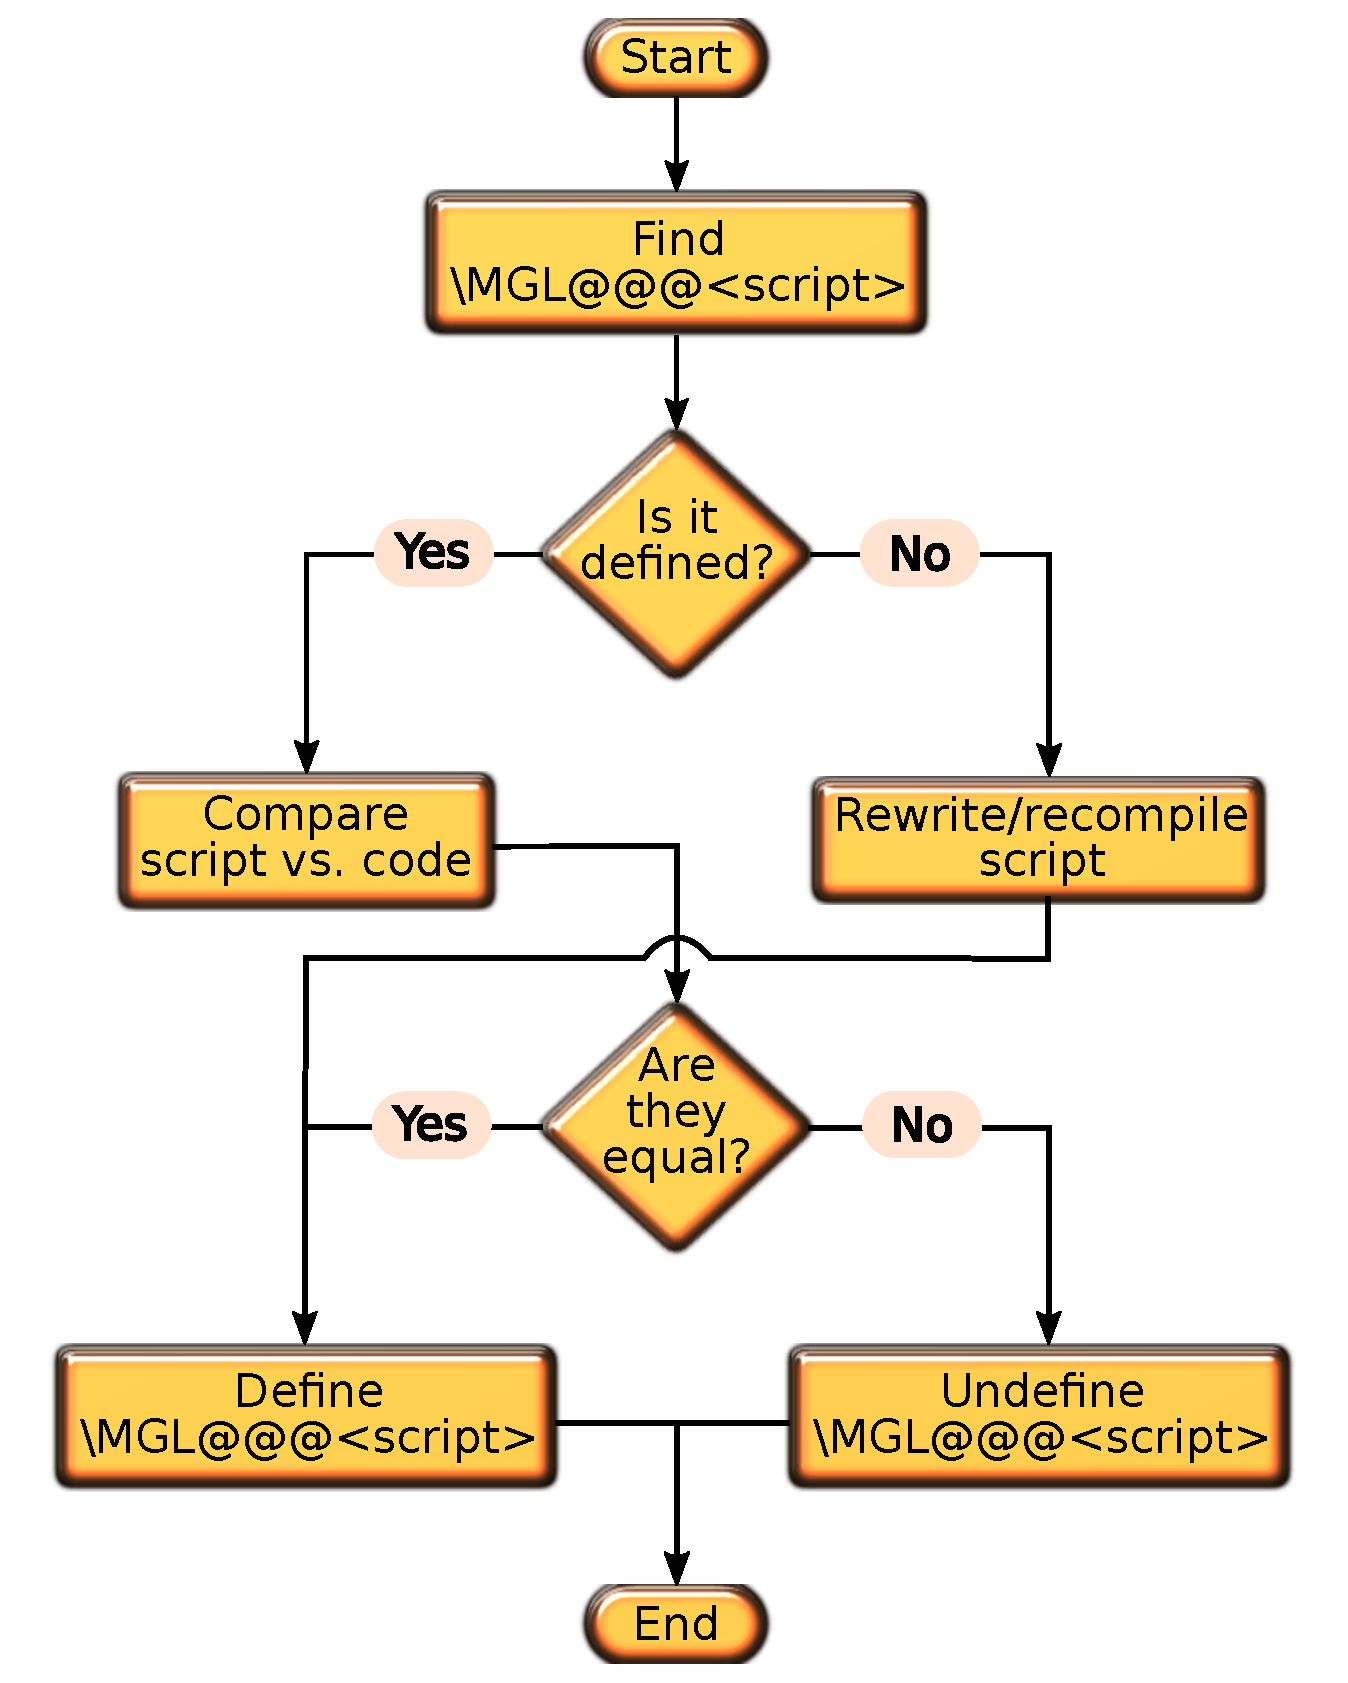
\includegraphics[scale=0.35]{Recompilation_decision}
%   \caption{The algorithm used by \textsf{\mglTeX} to decide which scripts recereate/recompile.}\label{fig: recompilation decision}
% \end{figure}
%
% The recompilation-decision mechanism can be fooled, however. The |mgl| environment and |\mglplot| command have the ability to automatically name scripts by means of the use of an internal counter, unless the |label| option is specified. Suppose the user wants to add a new |mgl| environment or |\mglplot| command exactly after the $(n-1)$th script, so the $n$th script will be the newly added, while the old $n$th will be the new $(n+1)$th, and so on, altering the original numbering. This will cause \textsf{\mglTeX} to compare the old $n$th script with the old $(n+1)$th, and so on, deciding they are different, so they will be recompiled.
%
% There are two ways to avoid this problem: The first one is to use the |label| option on the newly arrived; the second is to wrap a complete block of the document with the |\mgltexoff| and |\mgltexon| commands, avoiding recompilation and saving time. This last option will avoid the inclusion of the MGL graphics, so it is only recommended in case of the wrapped scripts being in their final version (not needing further modification), so there is no need of updating the corresponding graphics; then, when the document is compiled in its final version, the |\mgltexoff| and |\mgltexon| can be removed. However, the most recommended way of proceeding is to use the |\mglname| command to create a separated main script per document block (section, chapter, part, etc.), so that, if a new script disrupts the original numbering, \textsf{\mglTeX} will recompile only the scripts of the current block.
%
% There are situations when recompilation of a script has to be forced. For example, if the default quality has changed, but the script hasn't, \textsf{\mglTeX} won't recreate the corresponding graphic by its own initiative, because it won't detect any changes in the code. In order to force recompilation, the image of the corresponding script can be deleted: \textsf{\mglTeX} will detect this abscence in the next \LaTeX{} run and recompile.
%
% \section{Acknowledgements}
% \noindent \textsf{\mglTeX} was born as a small personal project. It has grown and mature under the constant suggestions and requests from Prof. Alexey Balakin.
%
% \section{Redistributing and modifying}
% \noindent The \emph{source code} of \textsf{\mglTeX} (.sty, .dtx, and .ins files) can be redistributed and/or modified under the terms of the GNU General Public License as published by the Free Software Foundation, either version 3 of the License, or (at your option) any later version. The \emph{documentation} of \textsf{\mglTeX} (.dvi, .ps, .pdf and other files) is licensed under the Creative Commons Attribution-NonCommercial-ShareAlike 3.0 Unported License. 
%
% \StopEventually{\PrintChanges\PrintIndex}
%
% \section{Implementation}
% \noindent This section documents the complete implementation of \textsf{\mglTeX}. It's main purpose is to facilitate the understanding and maintanance of the package's code. For the following, we use ``|@|'' in the name of macros the user should not modify; the prefix ``|MGL|'' is used to simulate a namespace, so the macros from \textsf{\mglTeX} won't interfere with the ones from other packages.
%
% \subsection{Initialization}
% \noindent We first define some macros that will serve different purposes on different parts of the package.
% \begin{macro}{\MGL@TeX@ext}
% Is used to determine whether the user has chosen to save graphics in \LaTeX/Tikz format.
%    \begin{macrocode}
\def\MGL@TeX@ext{.tex}
%    \end{macrocode}
% \end{macro}
%
% Now we declare the options |final| and |draft|, which are simply passed to the \textsf{graphicx} package.
%    \begin{macrocode}

\DeclareOption{draft}{%
  \PassOptionsToPackage{\CurrentOption}{graphicx}%
}
\DeclareOption{final}{%
  \PassOptionsToPackage{\CurrentOption}{graphicx}%
}
%    \end{macrocode}
%
% The next options are |on| and |off|. Since they are equivalent to the commands |\mgltexon| and |\mgltexoff|, respectively, instead of writing the same code twice (one time for the options and one time for the commands), we first define the commands and then make the options execute them. 
% \begin{macro}{\mgltexon}
% (Re)defines the commands to open, read, write and close scripts, and the command that includes MGL graphics.
%    \begin{macrocode}

\def\mgltexon{%
%    \end{macrocode}
% \begin{macro}{\MGL@openout}
% Opens a script for writing. It takes two arguments, the first being an output stream number, allocate by |\newwrite| (\TeX{} command), and the second being the path to the script.
%    \begin{macrocode}
  \def\MGL@openout##1##2{%
    \immediate\openout##1="##2"%
  }%
%    \end{macrocode}
% \end{macro}
% \begin{macro}{\MGL@openin}
% Opens a script for reading. It takes two arguments, the first being an input stream number, allocate by |\newread| (\TeX{} command), and the second being the path to the script.
%    \begin{macrocode}
  \def\MGL@openin##1##2{%
    \immediate\openin##1="##2"%
  }%
%    \end{macrocode}
% \end{macro}
% \begin{macro}{\MGL@write}
% Writes to a script opened with |\MGL@openout|. Its first argument is the output stream number of the script, and the second is the text to write.
%    \begin{macrocode}
  \def\MGL@write##1##2{%
    \immediate\write##1{##2}%
  }%
%    \end{macrocode}
% \end{macro}
% \begin{macro}{\MGL@read}
% Reads one line from a script opened with |\MGL@openin|. Its first argument is the input stream number of the script, and the second is a variable where the read text will be stored. The variable is first initialized as empty; if the end of the script has been reached, then there is nothing to read, so it remains empty; otherwise, one line is read and stored in the variable, locally supressing any end line character (|\endlinechar=-1|).
%    \begin{macrocode}
  \def\MGL@read##1##2{%
    \def##2{}%
    \ifeof##1\else%
      \bgroup%
      \endlinechar=-1%
      \immediate\global\read##1 to ##2%
      \egroup%
    \fi%
  }%
%    \end{macrocode}
% \end{macro}
% \begin{macro}{\MGL@closeout}
% Closes a script opened with |\MGL@openout|, whose stream number is passed as argument.
%    \begin{macrocode}
  \def\MGL@closeout##1{%
    \immediate\closeout##1%
  }
%    \end{macrocode}
% \end{macro}
% \begin{macro}{\MGL@closein}
% Closes a script opened with |\MGL@openin|, whose stream number is passed as argument.
%    \begin{macrocode}
  \def\MGL@closein##1{%
    \immediate\closein##1%
  }
%    \end{macrocode}
% \end{macro}
% \begin{macro}{\MGL@includegraphics}
% This is a quite sophisticated command. It is in charge of including the graphics created by \textsf{\mglTeX}.
%    \begin{macrocode}
  \def\MGL@includegraphics{%
%    \end{macrocode}
% First checks if the image exists. Note the |\MGL@dir| and |\MGL@graphics@dir| macros are set by the user with the |\mgldir| and |\mglgraphicsdir| commands, respectively, while |\MGL@script@name| stores the name of the script ---and thus the image--- executed, and |\MGL@graph@ext| is the extension chosen by the user to save the graphics.
%    \begin{macrocode}
    \IfFileExists{\MGL@dir\MGL@graphics@dir\MGL@script@name\MGL@graph@ext}{%
%    \end{macrocode}
% If the chosen extension is |.tex|, a \LaTeX/Tikz file has been created, which has to be simply included in the document; it will be automatically compiled by \LaTeX{}. (Observe we use the |\MGL@TeX@ext| macro defined above.)
%    \begin{macrocode}
      \ifx\MGL@graph@ext\MGL@TeX@ext%
        \include{\MGL@dir\MGL@graphics@dir\MGL@script@name\MGL@graph@ext}%
%    \end{macrocode}
% If the chosen extension is not |.tex|, a normal visual image has been created, so the |\includegraphics| command is invoked to deal with it. The options for this command (like |scale|, |angle|, etc.) are stored in the |\MGL@graph@keys| macro, which is defined by every environment or command that creates and compiles MGL scripts, according to the optional arguments the user has passed.
%    \begin{macrocode}
      \else%
        \expandafter\includegraphics\expandafter[\MGL@graph@keys]{%
          \MGL@dir\MGL@graphics@dir\MGL@script@name%
        }%
      \fi%
    }{%
%    \end{macrocode}
% If the requested image doesn't exist, the issue a warning message for the user, and print a warning framed box (``\textbf{MGL image not found}'') in the place the image should occupy.
%    \begin{macrocode}
      \PackageWarning{mgltex}{MGL image "\MGL@script@name" not found}%
      \fbox{%
        \centering%
        \bfseries\Huge%
        \begin{tabular}{c}MGL\\image\\not\\found\end{tabular}%
      }%
    }%
  }%
%    \end{macrocode}
% \end{macro}
% And here ends the |\mgltexon| command.
%    \begin{macrocode}
}
%    \end{macrocode}
% \end{macro}
%
% \begin{macro}{\mgltexoff}
% (Re)defines the same commands as |\mgltexon| in such a way they accept the same arguments, but do nothing. The exception is |\MGL@includegraphics| which, instead of doing nothing, prints a warning framed box (``\textbf{\mglTeX{} is off; no image included}'').
%    \begin{macrocode}
\def\mgltexoff{%
  \PackageWarning{mgltex}{mglTeX is off}%
  \def\MGL@openout##1##2{}%
  \def\MGL@openin##1##2{}%
  \def\MGL@write##1##2{}%
  \def\MGL@read##1##2{}%
  \def\MGL@closeout##1{}
  \def\MGL@closein##1{}
  \def\MGL@includegraphics{%
    \fbox{%
      \centering%
      \bfseries\Huge%
      \begin{tabular}{c}\mglTeX\\is off;\\no image\\included\end{tabular}%
    }%
  }%
}
%    \end{macrocode}
% \end{macro}
% Now we can declare the package options |on| and |off| so that they execute |\mgltexon| and |\mgltexoff|, respectively.
%    \begin{macrocode}
\DeclareOption{on}{\mgltexon}
\DeclareOption{off}{\mgltexoff}
%    \end{macrocode}
%
% The options |nocomments| and |comments| are equivalent to the commands |\mglnocomments| and |\mglcomments|, respectively, so, following the same logic as before, we first define the commands and make the options execute them.
% \begin{macro}{\@MGL@comments@}
% We will need a boolean switch to activate/deactivate commentaries later.
%    \begin{macrocode}

\newif\if@MGL@comments@
%    \end{macrocode}
% \end{macro}
% \begin{macro}{\mglnocomments} Declares |\@MGL@comments@| as false.
%    \begin{macrocode}
\def\mglnocomments{\@MGL@comments@false}
%    \end{macrocode}
% \end{macro}
% \begin{macro}{\mglcomments} Declares |\@MGL@comments@| as true.
%    \begin{macrocode}
\def\mglcomments{\@MGL@comments@true}
%    \end{macrocode}
% \end{macro}
% Now, the options call the respective commands.
%    \begin{macrocode}
\DeclareOption{nocomments}{\mglnocomments}
\DeclareOption{comments}{\mglcomments}
%    \end{macrocode}
%
% \begin{macro}{\mglscale}\begin{macro}{\MGL@scale}
% |\mglscale| sets the value of the |\MGL@scale| macro, which is used later to specify the default scaling for graphics. It only accepts integer values from $1$ to $9$, otherwise it issues a warning and restarts the scaling to $1$. In order to be able to check the validity of the value passed by the user, we first set the |\MGL@scale| macro to that value and test it with the |\ifcase| conditional; if the value is valid, we do nothing, but if it is invalid, we issue a warning and overwrite |\MGL@scale| to $1$.
%    \begin{macrocode}

\def\mglscale#1{
  \def\MGL@scale{#1}%
  \ifcase\MGL@scale\or\or\or\or\or\or\or\or\else%
    \PackageWarning{mgltex}{%
      Scaling value of \MGL@scale\space not allowed; using default (1)%
    }%
    \def\MGL@scale{1}%
  \fi%
}
%    \end{macrocode}
% \end{macro}\end{macro}
% The pacakage options |1x|, \ldots, |9x| just call |\mglscale| with the appropiate value.
%    \begin{macrocode}
\DeclareOption{1x}{\mglscale{1}}
\DeclareOption{2x}{\mglscale{2}}
\DeclareOption{3x}{\mglscale{3}}
\DeclareOption{4x}{\mglscale{4}}
\DeclareOption{5x}{\mglscale{5}}
\DeclareOption{6x}{\mglscale{6}}
\DeclareOption{7x}{\mglscale{7}}
\DeclareOption{8x}{\mglscale{8}}
\DeclareOption{9x}{\mglscale{9}}
%    \end{macrocode}
%
% \begin{macro}{\mglquality}\begin{macro}{\MGL@quality}
% |\mglquality| sets the value of the |\MGL@quality| macro, which is used later to specify the default quality for graphics. It only accepts integer values from $0$ to $8$ (the only ones defined by |MathGL|), otherwise it issues a warning and restarts to $2$ (the default for |MathGL|). In order to be able to check the validity of the value passed by the user, we first set the |\MGL@quality| macro to that value and test it with the |\ifcase| conditional; if the value is valid, we print an info message to the |.log| file about the characteristics of the chosen quality, but if it is invalid, we issue a warning and overwrite |\MGL@scale| to $2$.
% \end{macro}\end{macro}
%    \begin{macrocode}

\def\mglquality#1{%
  \def\MGL@quality{#1}%
  \ifcase\MGL@quality%
    \PackageInfo{mgltex}{%
      Quality 0: No face drawing (fastest)%
    }%
  \or%
    \PackageInfo{mgltex}{%
      Quality 1: No color interpolation (fast)%
    }%
  \or%
    \PackageInfo{mgltex}{%
      Quality 2: High quality (normal)%
    }%
  \or%
    \PackageInfo{mgltex}{%
      Quality 3: High quality with 3d primitives (not implemented yet)%
    }%
  \or%
    \PackageInfo{mgltex}{%
      Quality 4: No face drawing, direct bitmap drawing (low memory usage)%
    }%
  \or%
    \PackageInfo{mgltex}{%
      Quality 5: No color interpolation, direct bitmap drawing (low memory usage)%
    }%
  \or%
    \PackageInfo{mgltex}{%
      Quality 6: High quality, direct bitmap drawing (low memory usage)%
    }%
  \or%
    \PackageInfo{mgltex}{%
      Quality 7: High quality with 3d primitives, direct bitmap drawing (not implemented yet)%
    }%
  \or%
    \PackageInfo{mgltex}{%
      Quality 8: Draw dots instead of primitives (extremely fast)%
    }%
  \else%
    \PackageWarning{mgltex}{%
      Quality #1 not available; using default (2)%
    }%
    \def\MGL@quality{2}%
  \fi%
}
%    \end{macrocode}
% The package options |0q|, \ldots, |8q| just call |\mglquality| with the appropiate value.
%    \begin{macrocode}
\DeclareOption{0q}{\mglquality{0}}
\DeclareOption{1q}{\mglquality{1}}
\DeclareOption{2q}{\mglquality{2}}
\DeclareOption{3q}{\mglquality{3}}
\DeclareOption{4q}{\mglquality{4}}
\DeclareOption{5q}{\mglquality{5}}
\DeclareOption{6q}{\mglquality{6}}
\DeclareOption{7q}{\mglquality{7}}
\DeclareOption{8q}{\mglquality{8}}
%    \end{macrocode}
%
% \begin{macro}{\MGL@graph@ext}
% The following options set the default graphics extension, which is stored in the |\MGL@graph@ext| macro for later use.
%    \begin{macrocode}

\DeclareOption{eps}{\def\MGL@graph@ext{.eps}}
\DeclareOption{epsz}{\def\MGL@graph@ext{.epsz}}
\DeclareOption{epsgz}{\def\MGL@graph@ext{.eps.gz}}
\DeclareOption{bps}{\def\MGL@graph@ext{.bps}}
\DeclareOption{bpsz}{\def\MGL@graph@ext{.bpsz}}
\DeclareOption{bpsgz}{\def\MGL@graph@ext{.bps.gz}}
\DeclareOption{pdf}{\def\MGL@graph@ext{.pdf}}
\DeclareOption{png}{\def\MGL@graph@ext{.png}}
\DeclareOption{jpg}{\def\MGL@graph@ext{.jpg}}
\DeclareOption{jpeg}{\def\MGL@graph@ext{.jpeg}}
\DeclareOption{gif}{\def\MGL@graph@ext{.gif}}
\DeclareOption{tex}{\def\MGL@graph@ext{.tex}}
%    \end{macrocode}
% \end{macro}
%
% Any other option passed by the user is invalid, so an error message is issued.
%    \begin{macrocode}

\DeclareOption*{\@unknownoptionerror}
%    \end{macrocode}
%
% We now declare the default package options, and, finally, process the options the user specifies in the order they are introduced.
%    \begin{macrocode}

\ExecuteOptions{final,on,nocomments,1x,2q,eps}
\ProcessOptions*
%    \end{macrocode}
%
% \textsf{\mglTeX} requires the \textsf{keyval} package to define \meta{key}=\meta{value} options for the environments and commands; the \textsf{graphicx} package apports the facilities for inclusion of graphics, and the \textsf{verbatim} package is used as engine for the environments.
%    \begin{macrocode}

\RequirePackage{keyval}
\RequirePackage{graphicx}
\RequirePackage{verbatim}
%    \end{macrocode}
% The supported graphic formats are declared, and the |\verbatim@finish| command from the \textsf{verbatim} package is disabled to avoid it from writing a blank line at the end of every script (see subsection~\ref{subsection: warning}).
%    \begin{macrocode}
\DeclareGraphicsExtensions{%
  .eps,.epsz,.eps.gz,.bps,.bpsz,.bps.gz,.pdf,.png,.jpg,.jpeg,.gif%
}
\let\verbatim@finish\relax
%    \end{macrocode}
%
% \begin{macro}{\MGL@graph@keys}
% The main family of \meta{key}=\meta{value} pairs is defined. These pairs are common to every environment or command that produces graphics. Most of the \meta{key}'s are redefinitions of the optional arguments for the |\includegraphics| commands, so they are stored inside the |\MGL@graph@keys| macro, which is later passed to that command as optional argument by |\MGL@includegraphics|.
%    \begin{macrocode}

\define@key{MGL@keys}{bb}{\g@addto@macro\MGL@graph@keys{bb=#1,}}
\define@key{MGL@keys}{bbllx}{\g@addto@macro\MGL@graph@keys{bbllx=#1,}}
\define@key{MGL@keys}{bblly}{\g@addto@macro\MGL@graph@keys{bblly=#1,}}
\define@key{MGL@keys}{bburx}{\g@addto@macro\MGL@graph@keys{bburx=#1,}}
\define@key{MGL@keys}{bbury}{\g@addto@macro\MGL@graph@keys{bbury=#1,}}
\define@key{MGL@keys}{natwidth}{\g@addto@macro\MGL@graph@keys{natwidth=#1,}}
\define@key{MGL@keys}{natheight}{\g@addto@macro\MGL@graph@keys{natheight=#1,}}
\define@key{MGL@keys}{hiresbb}{\g@addto@macro\MGL@graph@keys{hiresbb=#1,}}
\define@key{MGL@keys}{viewport}{\g@addto@macro\MGL@graph@keys{viewport=#1,}}
\define@key{MGL@keys}{trim}{\g@addto@macro\MGL@graph@keys{trim=#1,}}
\define@key{MGL@keys}{angle}{\g@addto@macro\MGL@graph@keys{angle=#1,}}
\define@key{MGL@keys}{origin}{\g@addto@macro\MGL@graph@keys{origin=#1,}}
\define@key{MGL@keys}{width}{\g@addto@macro\MGL@graph@keys{width=#1,}}
\define@key{MGL@keys}{height}{\g@addto@macro\MGL@graph@keys{height=#1,}}
\define@key{MGL@keys}{totalheight}{\g@addto@macro\MGL@graph@keys{totalheight=#1,}}
\define@key{MGL@keys}{keepaspectratio}[true]{%
  \g@addto@macro\MGL@graph@keys{keepaspectratio=#1,}%
}
\define@key{MGL@keys}{scale}{\g@addto@macro\MGL@graph@keys{scale=#1,}}
\define@key{MGL@keys}{clip}[true]{\g@addto@macro\MGL@graph@keys{clip=#1,}}
\define@key{MGL@keys}{draft}[true]{\g@addto@macro\MGL@graph@keys{draft=#1,}}
\define@key{MGL@keys}{type}{\g@addto@macro\MGL@graph@keys{type=#1,}}
\define@key{MGL@keys}{ext}{\g@addto@macro\MGL@graph@keys{ext=#1,}}
\define@key{MGL@keys}{read}{\g@addto@macro\MGL@graph@keys{read=#1,}}
\define@key{MGL@keys}{command}{\g@addto@macro\MGL@graph@keys{command=#1,}}
%    \end{macrocode}
% \end{macro}
% \begin{macro}{\MGL@graph@ext}
% Stores the default extension for the creation of the graphics.
%    \begin{macrocode}
\define@key{MGL@keys}{imgext}{\def\MGL@graph@ext{.#1}}
%    \end{macrocode}
% \end{macro}
%
% \begin{macro}{\@MGL@lineno@}
% The only \meta{key}=\meta{value} pair needed for verbatim-like environments and commands is the one for the |lineno| option, which sets the value of the |\@MGL@lineno@| boolean macro.
%    \begin{macrocode}

\newif\if@MGL@lineno@
\define@key{MGL@verb@keys}{lineno}[true]{\csname @MGL@lineno@#1\endcsname}
%    \end{macrocode}
% \end{macro}
%
% \begin{macro}{\MGL@main@script@name}
% \noindent This macro stores the name of the of the document's main script. It is initialized to the name of the \LaTeX{} document.
%    \begin{macrocode}

\edef\MGL@main@script@name{\jobname}
%    \end{macrocode}
% \end{macro}
%
% \begin{macro}{\MGL@dir}
% This is the \textsf{\mglTeX} main working directory. By default, it is defined to empty, so it points to the path of the \LaTeX{} document.
%    \begin{macrocode}

\def\MGL@dir{}
%    \end{macrocode}
% \end{macro}
% \begin{macro}{\MGL@scripts@dir}
% The subdirectory inside |\MGL@dir| where all MGL scripts will be created.
%    \begin{macrocode}
\def\MGL@scripts@dir{}
%    \end{macrocode}
% \end{macro}
% \begin{macro}{\MGL@graphics@dir}
% The subdirectory inside |\MGL@dir| where all MGL graphics will be created.
%    \begin{macrocode}
\def\MGL@graphics@dir{}
%    \end{macrocode}
% \end{macro}
% \begin{macro}{\MGL@backups@dir}
% The subdirectory inside |\MGL@dir| where all backups of scripts will be created.
%    \begin{macrocode}
\def\MGL@backups@dir{}
%    \end{macrocode}
% \end{macro}
% \begin{macro}{\MGL@paths}
% This is a list of paths where extracted and external scripts will be searched for by the |\mglgraphics| and |\mglinclude| commands. Since extracted scripts are created inside |\MGL@dir\MGL@scripts@dir| and |\MGL@dir\MGL@backups@dir|, this directories are included.
%    \begin{macrocode}
\def\MGL@paths{\MGL@dir\MGL@scripts@dir,\MGL@dir\MGL@backups@dir}
%    \end{macrocode}
% \end{macro}
%
% We set some additional staff that will be used later.
% \begin{macro}{\MGL@main@stream}
% The output stream for the document's main script.
%    \begin{macrocode}

\newwrite\MGL@main@stream
%    \end{macrocode}
% \end{macro}
% \begin{macro}{\MGL@out@stream}
% The output stream for scripts other than the main one.
%    \begin{macrocode}
\newwrite\MGL@out@stream
%    \end{macrocode}
% \end{macro}
% \begin{macro}{\MGL@in@stream}
% The input stream for scripts other than the main one.
%    \begin{macrocode}
\newread\MGL@in@stream
%    \end{macrocode}
% \end{macro}
% \begin{macro}{MGL@script@no}
% The internal counter used by environments like |mgl| and commands like |\mglplot| to automatically name scripts.
%    \begin{macrocode}
\newcounter{MGL@script@no}
%    \end{macrocode}
% \end{macro}
% \begin{macro}{MGL@line@no}
% The counter used for verbatim-like environments and commands to numerate the lines of code.
%    \begin{macrocode}
\newcounter{MGL@line@no}
%    \end{macrocode}
% \end{macro}
% \begin{macro}{MGL@verb@script@no}
% The counter used to numerate verbatim-written scripts with the |\listofmglscripts| command.
%    \begin{macrocode}
\newcounter{MGL@verb@script@no}
%    \end{macrocode}
% \end{macro}
% \begin{macro}{\@MGL@list@script@}
% The boolean switch used to determine whether to add a verbatim-written script to the \emph{list of MGL scripts}.
%    \begin{macrocode}
\newif\if@MGL@list@script@
%    \end{macrocode}
% \end{macro}
% \begin{macro}{\l@MGL@script}
% Finally, the style for the leaders associating script name and page number in the \emph{list of MGL scripts}.
%    \begin{macrocode}
\def\l@MGL@script{\@dottedtocline{1}{0em}{1.5em}}
%    \end{macrocode}
% \end{macro}
%
% \subsection{Anatomy of environments and commands}\label{subsection: anatomy}
% \noindent Many of the environments and commands defined by \textsf{\mglTeX} are based on the same pieces of code. So, in order to avoid repetition of commands, we use the concept of \emph{anatomy of environments and commands}, which is basically the idea of taking repetitive pieces of code and enclose them into macros which can later be used.
%
% \begin{macro}{\MGL@setkeys}
% This command recieves two arguments: a family of \meta{key}=\meta{value} pairs, like |MGL@keys|, and a list of such pairs. It first cleans the |\MGL@graph@keys| macro, and the process the list of pairs.
%    \begin{macrocode}

\def\MGL@setkeys#1#2{%
  \def\MGL@graph@keys{}%
  \setkeys{#1}{#2}%
}
%    \end{macrocode}
% \end{macro}
%
% \begin{macro}{\MGL@codes}
% This macro changes the category codes of all special characters (like |\|, |$|, etc.) to $12$ (other), so they don't have any special meaning and can be processed as normal text. The exception is the new line character (|^^M|), which is kept active for compatibility with the \textsf{verbatim} package.
%    \begin{macrocode}

\def\MGL@codes{%
  \let\do\@makeother\dospecials%
  \catcode`\^^M\active%
}
%    \end{macrocode}
% \end{macro}
%
% \begin{macro}{\MGL@document@scripts}
% A macro to store the names of the scripts created or compiled in the document.
%    \begin{macrocode}

\def\MGL@document@scripts{}
%    \end{macrocode}
% \end{macro}
% \begin{macro}{\MGL@set@script@name}\begin{macro}{\MGL@script@name}
% |\MGL@set@script@name| recieves the name of a script without extension as argument, defines |\MGL@script@name| as that name, and checks if it has already been created or compiled, by comparing it with the names already stored in |\MGL@document@scripts|; if it's there already, warns the user. Finally, adds the name of the script to |\MGL@document@scripts|.
%    \begin{macrocode}
\def\MGL@set@script@name#1{%
  \edef\MGL@script@name{#1}%
  \@for\MGL@temp@a:=\MGL@document@scripts\do{%
    \ifx\MGL@temp@a\MGL@script@name%
      \PackageWarning{mgltex}{Multiple MGL scripts named "\MGL@script@name.mgl"}%
    \fi%
  }%
  \g@addto@macro\MGL@document@scripts{\MGL@script@name,}%
}
%    \end{macrocode}
% \end{macro}\end{macro}
%
% \begin{macro}{\MGL@unchanged}
% This command defines the ``switch'' |\MGL@@@|\meta{script}, where \meta{script} is passed as argument, which indicates the script \meta{script}|.mgl| has not changed. This command has to be written to the |.aux| file to be preserved from compilation to compilation.
%    \begin{macrocode}

\def\MGL@unchanged#1{%
  \global\@namedef{MGL@@@#1}{}%
}
%    \end{macrocode}
% \end{macro}
%
% \begin{macro}{\MGL@process@script}
% It checks whether the ``switch'' |\MGL@@@\MGL@script@name| is undefined, in which case executes its first argument. If the switch is defined, it checks if the corresponding image has been created; if so, it executes its second argument; otherwise, the first one.
%    \begin{macrocode}

\def\MGL@process@script#1#2{%
  \@ifundefined{MGL@@@\MGL@script@name}{%
    #1%
  }{%
    \IfFileExists{\MGL@dir\MGL@graphics@dir\MGL@script@name\MGL@graph@ext}{%
      #2%
    }{%
      #1%
    }%
  }%
}
%    \end{macrocode}
% \end{macro}
%
% \begin{macro}{\MGL@def@for@loop}\begin{macro}{\MGL@for}
% |\MGL@def@for@loop| defines the command |\MGL@for| which is similar to the |\@for| command from the \LaTeX{} kernel, with the only exception that, instead of iterating over comma-separated lists, it can iterate over lists of items with any kind of separator, which is passed as argument of |\MGL@def@for@loop|. The body of this command is copied from the definition code of |\@for|, extracted from \emph{The \LaTeXe{} Sources} document, replacing the ``|,|'' by ``|#1|''. Note that |\MGL@for| is used only by the |\mglplot| command, but it has been included as part of the \emph{anatomy of environments and commands} to keep cleanness because it is quite long code.
%    \begin{macrocode}

\def\MGL@def@for@loop#1{%
  \long\def\MGL@for##1:=##2\do##3{%
    \expandafter\def\expandafter\@fortmp\expandafter{##2}%
    \ifx\@fortmp\@empty\else%
      \expandafter\MGL@forloop##2#1\@nil#1\@nil\@@##1{##3}%
    \fi%
  }%
  \long\def\MGL@forloop##1#1##2#1##3\@@##4##5{%
    \def##4{##1}%
    \ifx##4\@nnil\else%
      ##5\def##4{##2}%
      \ifx##4\@nnil\else%
        ##5\MGL@iforloop##3\@@##4{##5}%
      \fi%
    \fi%
  }%
  \long\def\MGL@iforloop##1#1##2\@@##3##4{%
    \def##3{##1}%
    \ifx##3\@nnil%
      \expandafter\@fornoop%
    \else%
      ##4\relax\expandafter\MGL@iforloop%
    \fi%
    ##2\@@##3{##4}%
  }%
}
%    \end{macrocode}
% The default |\MGL@for| loop iterates over |^^J|-separated lists, i.e, \meta{new line}-character-lists.
%    \begin{macrocode}
\MGL@def@for@loop{^^J}
%    \end{macrocode}
% \end{macro}\end{macro}
%
% \begin{macro}{\MGL@compare@code}
% |\MGL@compare@code| is in charge of comparing the user's MGL code, embedded within \textsf{\mglTeX} environments, with its corresponding extracted script. For that purpose, the |\verbatim@processline| and |\verbatim@finish| commands from the \textsf{verbatim} package are redefined.
%    \begin{macrocode}

\def\MGL@compare@code#1{%
%    \end{macrocode}
% \begin{macro}{\MGL@next}
% This macro is called at the end of environments that use the |\MGL@compare@code| macro, and performs the ending actions of the comparision process, which are closing the |\MGL@in@stream| and writing the |\MGL@unchanged{\MGL@script@name}| to the |.aux| file. If during the comparison process a difference in the code is found, |\MGL@next| is redefined to only close the |\MGL@in@stream|.
%    \begin{macrocode}
  \def\MGL@next{%
    \MGL@closein\MGL@in@stream%
    \MGL@write\@auxout{\string\MGL@unchanged{\MGL@script@name}}%
  }%
%    \end{macrocode}
% \end{macro}
% The |\verbatim@processline| command is redefined to read from the input stream to a temporary variable (|\MGL@temp@a|), and compare it with one line of code in the \LaTeX{} document, which is stored in another temporary variable (|\MGL@temp@b|). In case they are not equal, the |\MGL@next| macro is redefined to only close the input stream, and |\verbatim@processline| is redefine again to do nothing (a little speed-up).
%    \begin{macrocode}
  \def\verbatim@processline{%
    \MGL@read\MGL@in@stream{\MGL@temp@a}%
    \edef\MGL@temp@b{\the\verbatim@line}%
    \ifx\MGL@temp@a\MGL@temp@b\else%
      \def\MGL@next{\MGL@closein\MGL@in@stream}%
      \def\verbatim@processline{}%
    \fi%
  }%
%    \end{macrocode}
% The |\verbatim@finish| macro, which is called at the end of the environment, is also redefined to perform one last read of the input stream, and then check if the end of file has been reached; if it hasn't, then, despite the end of the environment has been reached ---thus the end of code---, there is still code inside the script, so there are differences between them, and |\MGL@next| has to be redefined to do nothing but close the input stream.
%    \begin{macrocode}
  \def\verbatim@finish{%
    \MGL@read\MGL@in@stream{\MGL@temp@a}%
    \ifeof\MGL@in@stream\else%
      \def\MGL@next{\MGL@closein\MGL@in@stream}%
    \fi%
  }%
%    \end{macrocode}
% Finally, the input stream is opened, and the comparison is started by calling |\verbatim@start|.
%    \begin{macrocode}
  \MGL@openin\MGL@in@stream{#1}%
  \verbatim@start%
}
%    \end{macrocode}
% \end{macro}
%
% \begin{macro}{\MGL@write@funcs}
% This macro is used only by the |mglfunc| environment. Its only purpose is to store the commands to insert MGL functions in the main script, and is called at the end of the document or when the |\mglname| command is used. For now, we only ask it to write the |stop| command\footnote{Note the |stop| command is unnecesary in newer versions of the MGL language, but it is kept in \textsf{\mglTeX} for compatibility and for elegance.} that separates the section of scripts from the section of functions in the main script.
%    \begin{macrocode}

\def\MGL@write@funcs{\MGL@write\MGL@main@stream{stop^^J}}
%    \end{macrocode}
% \end{macro}
% \begin{macro}{\MGL@func}
% This is the command that writes the MGL functions. It is intended to be stored inside |\MGL@write@funcs|. It opens the backup file of the MGL function whose name is passed as argument (and has been created by a |mglfunc| environment), and then calls |\MGL@@func| to transcript from that file, line by line, to the main script.
%    \begin{macrocode}
\def\MGL@func#1{%
  \MGL@openin\MGL@in@stream{\MGL@dir\MGL@backups@dir#1.mgl}%
  \MGL@@func%
}
%    \end{macrocode}
% \end{macro}
% \begin{macro}{\MGL@@func}
% This command transcripts only one line from backup file of a MGL function to the main script. It calls itself recursively until the end of the backup.
%    \begin{macrocode}
\def\MGL@@func{%
%    \end{macrocode}
% It first reads from the input stream to the |\MGL@temp@a| temporary variable.
%    \begin{macrocode}
  \MGL@read\MGL@in@stream{\MGL@temp@a}%
%    \end{macrocode}
% If the end of the file has been reached, the stream is closed.
%    \begin{macrocode}
  \ifeof\MGL@in@stream%
    \MGL@closein\MGL@in@stream%
%    \end{macrocode}
% If the end of file hasn't been reached, |\MGL@temp@a| is written to the main script, and |\MGL@@func| is called recursively.
%    \begin{macrocode}
  \else%
    \MGL@write\MGL@main@stream{\MGL@temp@a}%
    \expandafter\MGL@@func%
  \fi%
}
%    \end{macrocode}
% \end{macro}
%
% \begin{macro}{\MGL@set@verbatim@code}
% This command sets the parameters for verbatim-like environments and commands.
%    \begin{macrocode}

\def\MGL@set@verbatim@code{%
%    \end{macrocode}
% The following is standard stuff for verbatim-like environments and commands.
%    \begin{macrocode}
  \if@minipage\else\vskip\parskip\fi%
  \leftskip\@totalleftmargin\rightskip\z@skip%
  \parindent\z@\parfillskip\@flushglue\parskip\z@%
  \@@par%
  \def\par{%
    \if@tempswa%
      \leavevmode\null\@@par\penalty\interlinepenalty%
    \else%
      \@tempswatrue%
      \ifhmode\@@par\penalty\interlinepenalty\fi%
    \fi%
  }%
  \obeylines%
  \let\do\@makeother\dospecials%
  \verbatim@font%
  \frenchspacing%
  \everypar\expandafter{\the\everypar\unpenalty}%
%    \end{macrocode}
% If there are no lines of MGL code, instead of issuing an error, we display a package warning.
%    \begin{macrocode}
  \def\@noitemerr{\PackageWarning{mglTeX}{Empty MGL script}}%
%    \end{macrocode}
% The space between the end of the label box and the text of the first item (|\labelsep|) is set to |1em|, while the separation between items (|\itemsep|) is set to zero.
%    \begin{macrocode}
  \labelsep1em%
  \itemsep\z@%
%    \end{macrocode}
% Since we want the lines of code to be broken between words, but verbatim spaces are unbreakable, we trick \LaTeX{} by inserting a breakable spaces (|\space|) instead.
%    \begin{macrocode}
  \def\@xobeysp{\space}\@vobeyspaces%
%    \end{macrocode}
% However, \LaTeX{} still resists breaking lines as much as possible in order to preserve the shape of paragraphs, so we tell it it's OK not to do so by setting the badness tolerance before hyphenation (|\pretolerance|) and the badness above which bad hboxes will be shown (|\hbadness|) to the maximum value of $10000$ (|\@M|).
%    \begin{macrocode}
  \pretolerance\@M%
  \hbadness\@M%
%    \end{macrocode}
% In order to achieve the desired indentation of broken lines, we use the following trick: We increase the |\leftskip| parameter by the amount specified by |\mglbreakindent|, so that lines will be indented; but then we decrease the |\itemindent| parameter by the same amount so the first line won't be indented.
%    \begin{macrocode}
  \advance\leftskip\mglbreakindent%
  \itemindent-\mglbreakindent%
}
%    \end{macrocode}
% \end{macro}
%
% \begin{macro}{\MGL@line@sep}
% This is the separator displayed at the beginning and ending of the |mglblock| and |mglverbatim| environments, to distinguish the MGL code from the normal text. Its definition is similar to the one of the |\dotfill| command, which can be found in \emph{The \LaTeXe{} Sources} document, but |\nopagebreak| commands have been added to avoid unaesthetic page breaking before and after the separators.
%    \begin{macrocode}

\def\MGL@line@sep{%
  \nopagebreak%
  \leavevmode\cleaders\hrule height\mgllinethickness\hfill\kern\z@%
  \nopagebreak%
}
%    \end{macrocode}
% \end{macro}
% \begin{macro}{\MGL@dash@sep}
% This is the separator displayed at the begginning and ending of the |mglcomments| environment, when it is allowed to be displayed.
%    \begin{macrocode}
\def\MGL@dash@sep{%
  \nopagebreak%
  \leavevmode\cleaders\hb@xt@\mgldashwidth{\hss-\hss}\hfill\kern\z@%
  \nopagebreak%
}
%    \end{macrocode}
% \end{macro}
%
% \subsection{Environments for MGL code embedding}
% \noindent For the following, we agree that if a macro is required by an environment, and it hasn't been already defined, it will be defined between the commands that start and end such environment; also the command's name will have the environment's name as prefix.
%
% \begin{environment}{mgl}
% This environment has to transcript its contents to the document's main script, and create a backup of the code simultaneously; the backup is used to detect changes in following compilations.
% \begin{macro}{\mgl}
% The command that starts the |mgl| environment. It is called by the |\begin{mgl}| command.
%    \begin{macrocode}

\newcommand\mgl[1][]{%
%    \end{macrocode}
% We define an additional \meta{key}=\meta{value} pair in the main family of pairs, corresponding to the |label| option for this environment. This definition is local because we don't want to be valid outside the environment.
%    \begin{macrocode}
  \define@key{MGL@keys}{label}{\def\MGL@script@name{##1}}%
%    \end{macrocode}
% The list of comma-separated options is processed.
%    \begin{macrocode}
  \MGL@setkeys{MGL@keys}{#1}%
%    \end{macrocode}
% If the user hasn't used the |label| option, the automatic naming mechanism is called. Note that |\MGL@main@script@name| is set using the |\mglname| command.
%    \begin{macrocode}
  \@ifundefined{MGL@script@name}{%
    \stepcounter{MGL@script@no}%
    \edef\MGL@script@name{\MGL@main@script@name-MGL-\arabic{MGL@script@no}}%
  }{}%
%    \end{macrocode}
% We use the |\MGL@set@script@name| to test whether the given name has already been used.
%    \begin{macrocode}
  \MGL@set@script@name{\MGL@script@name}%
%    \end{macrocode}
% |\MGL@codes| is used to change the codes of special characters.
%    \begin{macrocode}
  \MGL@codes%
%    \end{macrocode}
% |\MGL@process@script| is used to test whether the code has changed or not the last time \LaTeX{} has been executed. If it has changed, we call the |\mgl@write@script| command to (re)write the code; otherwise, the code is scanned again by asking |\MGL@compare@code| to perform a comparison on the backup file, in order to determine whether the code has changed now.
%    \begin{macrocode}
  \MGL@process@script{%
    \mgl@write@script%
  }{%
    \MGL@compare@code{\MGL@dir\MGL@backups@dir\MGL@script@name.mgl}%
  }%
}
%    \end{macrocode}
% \end{macro}
% \begin{macro}{\mgl@write@script}
% (Re)writes the contents of the |mgl| environment.
%    \begin{macrocode}
\def\mgl@write@script{%
%    \end{macrocode}
% \begin{macro}{\MGL@next}
% It contains the actions to perform immediately after the end of |\mgl@write@script|. They are close the output stream; write in the main script the commands to save the image, and to reset the initial values for all MGL parameters and clear the image; finally, write |\MGL@unchanged{\MGL@script@name}| in the |.aux| file.
%    \begin{macrocode}
  \def\MGL@next{%
    \MGL@closeout\MGL@out@stream%
    \MGL@write\MGL@main@stream{%
      write '\MGL@dir\MGL@graphics@dir\MGL@script@name\MGL@graph@ext'^^J%
      ^^Jreset^^J%
    }%
    \MGL@write\@auxout{\string\MGL@unchanged{\MGL@script@name}}%
  }%
%    \end{macrocode}
% \end{macro}
% Now we redefine the |\verbatim@processline| macro to write |\the\verbatim@line| to the main script and to the backup file.
%    \begin{macrocode}
  \def\verbatim@processline{%
    \MGL@write\MGL@main@stream{\the\verbatim@line}%
    \MGL@write\MGL@out@stream{\the\verbatim@line}%
  }%
%    \end{macrocode}
% Before writing the MGL code of the environment, we set the default quality.
%    \begin{macrocode}
  \MGL@write\MGL@main@stream{quality \MGL@quality}%
%    \end{macrocode}
% We open the backup file in the output stream.
%    \begin{macrocode}
  \MGL@openout\MGL@out@stream{\MGL@dir\MGL@backups@dir\MGL@script@name.mgl}%
%    \end{macrocode}
% The transcription process starts by calling the |\verbatim@start| command.
%    \begin{macrocode}
  \verbatim@start%
}
%    \end{macrocode}
% \end{macro}
% \begin{macro}{\endmgl}
% The command that ends the |mgl| evironment. It is called by the |\end{mgl}| command. It simply calls |\MGL@next| to execute the final actions, and |\MGL@includegraphics| to insert the corresponding image. Note that |\MGL@next| performs different actions depending on whether |\MGL@process@script| calls |\mgl@write@script| or |\MGL@compare@code|, both of which define |\MGL@next| differently.
%    \begin{macrocode}
\def\endmgl{%
  \MGL@next%
  \MGL@includegraphics%
}
%    \end{macrocode}
% \end{macro}
% \end{environment}
%
% \begin{environment}{mgladdon}
% This environment only writes its contents to the document's main script, so no backup is created, nor compilation or inclusion of graphics.
% \begin{macro}{\mgladdon}
% Since this environment doesn't produce any output in the \LaTeX{} document, we start a \emph{space hack} by calling |\@bsphack|. We set the appropiate category codes with |\MGL@codes|; the |\verbatim@processline| is redefined to transcript |\the\verbatim@line| to the main script; finally, the |\verbatim@start| command starts the transcription process.
%    \begin{macrocode}

\def\mgladdon{%
  \@bsphack%
  \MGL@codes%
  \def\verbatim@processline{%
    \MGL@write\MGL@main@stream{\the\verbatim@line}%
  }%
  \verbatim@start%
}
%    \end{macrocode}
% \end{macro}
% \begin{macro}{\endmgladdon}
% The environment ends by closing the \emph{space hack} with |\@esphack|.
%    \begin{macrocode}
\def\endmgladdon{\@esphack}
%    \end{macrocode}
% \end{macro}
% \end{environment}
%
% \begin{environment}{mglfunc}
% This environment is used to define MGL functions inside the document's main script. Instead of writing directly to the main script, which would cause the MGL parser to end the execution of that script, it writes to a backup file which is later transcript before closing the main script.
% \begin{macro}{\mglfunc}
% It starts the |mglfunc| environment.
%    \begin{macrocode}

\newcommand\mglfunc[2][0]{%
%    \end{macrocode}
% Once again, since this command doesn't produce any output in the \LaTeX{} document, we use a \emph{space hack}.
%    \begin{macrocode}
  \@bsphack%
%    \end{macrocode}
% Although MGL functions and normal scripts are diferent in nature, in the sense that the first don't produce graphics by themselves, we have to check whether the function is being named as another script, because otherwise we run the risk of overwriting a backup file or confusing the parser.
%    \begin{macrocode}
  \MGL@set@script@name{#2}%
%    \end{macrocode}
% The instruction to transcript from the backup file to the main stream is stored in |\MGL@write@funcs| (see subsection \ref{subsection: anatomy}).
%    \begin{macrocode}
  \g@addto@macro\MGL@write@funcs{\MGL@func{#2}}%
%    \end{macrocode}
% The codes for special characters are set.
%    \begin{macrocode}
  \MGL@codes%
%    \end{macrocode}
% The |\verbatim@processline| command is redefined to write |\the\verbatim@line| to the backup file.
%    \begin{macrocode}
  \def\verbatim@processline{\MGL@write\MGL@out@stream{\the\verbatim@line}}%
%    \end{macrocode}
% The backup file is opened for writing.
%    \begin{macrocode}
  \MGL@openout\MGL@out@stream{\MGL@dir\MGL@backups@dir\MGL@script@name.mgl}%
%    \end{macrocode}
% The head of the function is written.
%    \begin{macrocode}
  \MGL@write\MGL@out@stream{func '\MGL@script@name' #1}%
%    \end{macrocode}
% The writing process is started.
%    \begin{macrocode}
  \verbatim@start%
}
%    \end{macrocode}
% \end{macro}
% \begin{macro}{\endmglfunc}
% It ends the |mglfunc| environment.
%    \begin{macrocode}
\def\endmglfunc{%
%    \end{macrocode}
% The end of the function is written.
%    \begin{macrocode}
  \MGL@write\MGL@out@stream{return^^J}%
%    \end{macrocode}
% The output stream is closed.
%    \begin{macrocode}
  \MGL@closeout\MGL@out@stream%
%    \end{macrocode}
% The \emph{space hack} is terminated.
%    \begin{macrocode}
  \@esphack%
}%
%    \end{macrocode}
% \end{macro}
% \end{environment}
%
% \begin{environment}{mglcode}
% This environment also checks for changes on the code, but, since it writes to its own script, there is no need to create a backup file (the check is performed using the script itself).
% \begin{macro}{\mglcode}
% It starts the |mglcode| environment. Its anatomy is similar to that of the |\mgl| command.
%    \begin{macrocode}

\newcommand\mglcode[2][]{%
  \MGL@setkeys{MGL@keys}{#1}%
  \MGL@set@script@name{#2}%
  \MGL@codes%
  \MGL@process@script{%
    \mglcode@write@script%
  }{%
    \MGL@compare@code{\MGL@dir\MGL@scripts@dir\MGL@script@name.mgl}%
  }%
}
%    \end{macrocode}
% \end{macro}
% \begin{macro}{\mglcode@write@script}
% This command takes care of creating the script for the |mglcode| environment.
%    \begin{macrocode}
\def\mglcode@write@script{%
%    \end{macrocode}
% \begin{macro}{\MGL@next}
% It performs the actions immediately following the end of |\mglcode@write@script|.
%    \begin{macrocode}
  \def\MGL@next{%
%    \end{macrocode}
% The output stream is closed.
%    \begin{macrocode}
    \MGL@closeout\MGL@out@stream%
%    \end{macrocode}
% The |\MGL@unchanged{\MGL@script@name}| command is written to the |.aux| file.
%    \begin{macrocode}
    \MGL@write\@auxout{\string\MGL@unchanged{\MGL@script@name}}%
%    \end{macrocode}
% The script compilation instruction is written to the terminal.
%    \begin{macrocode}
    \MGL@write{18}{%
      mglconv -q \MGL@quality\space -S \MGL@scale\space%
      -s "\MGL@dir\MGL@scripts@dir\mglcommonscriptname.mgl"\space%
      -o "\MGL@dir\MGL@graphics@dir\MGL@script@name\MGL@graph@ext"\space%
      "\MGL@dir\MGL@scripts@dir\MGL@script@name.mgl"%
    }%
  }%
%    \end{macrocode}
% \end{macro}
% The |\verbatim@processline| command is redefined so it writes |\the\verbatim@line| to the output stream.
%    \begin{macrocode}
  \def\verbatim@processline{\MGL@write\MGL@out@stream{\the\verbatim@line}}%
%    \end{macrocode}
% The script is opened for writing in the output stream.
%    \begin{macrocode}
  \MGL@openout\MGL@out@stream{\MGL@dir\MGL@scripts@dir\MGL@script@name.mgl}%
%    \end{macrocode}
% The writing process is started by calling the |\verbatim@start| command.
%    \begin{macrocode}
  \verbatim@start%
}
%    \end{macrocode}
% \end{macro}
% \begin{macro}{\endmglcode}
% It ends the |mglcode| environment. |\MGL@next| is called to perform the final actions and |\MGL@includegraphics| is called to insert the corresponding image. Once more, |\MGL@next| has different meanings depending on whether |\MGL@process@script| branches to |\MGL@compare@code| or |\mglcode@write@script|.
%    \begin{macrocode}
\def\endmglcode{%
  \MGL@next%
  \MGL@includegraphics%
}
%    \end{macrocode}
% \end{macro}
% \end{environment}
% \begin{environment}{mglscript}
% The only function of this environment is to write its contents to a script; no image is created. It has been considered that scanning the code looking for changes is as much operation-expensive as simply writing the code, so it has been decided that this environment (over)writes the script everytime it's executed, without performing any check.
% \begin{macro}{\mglscript}
% Starts the environment. Its anatomy is similar to the previous environments. Since no output is written to the \LaTeX{} document, a \emph{space hack} is used.
%    \begin{macrocode}

\def\mglscript#1{%
  \@bsphack%
  \MGL@set@script@name{#1}%
  \MGL@codes%
  \def\verbatim@processline{\MGL@write\MGL@out@stream{\the\verbatim@line}}%
  \MGL@openout\MGL@out@stream{\MGL@dir\MGL@scripts@dir\MGL@script@name.mgl}%
  \verbatim@start%
}
%    \end{macrocode}
% \end{macro}
% \begin{macro}{\endmglscript}
% It ends the |mglscript| environment. The \emph{space hack} ends here, too.
%    \begin{macrocode}
\def\endmglscript{%
  \MGL@closeout\MGL@out@stream%
  \@esphack%
}
%    \end{macrocode}
% \end{macro}
% \end{environment}
%
% \begin{environment}{mglcommon}
% This environment doesn't require any backup file nor any scanning for changes. Although the user sets the name of the script by redifining |\mglcommonscriptname|, it is necessary to perform a check of the name, just in case a name has been inadvertedly repeated.
% \begin{macro}{\mglcommon}
% Starts the |mglcommon| environment.
%    \begin{macrocode}

\def\mglcommon{%
  \@bsphack%
  \MGL@set@script@name{\mglcommonscriptname}%
  \MGL@codes%
  \def\verbatim@processline{\MGL@write\MGL@out@stream{\the\verbatim@line}}%
  \MGL@openout\MGL@out@stream{\MGL@dir\MGL@scripts@dir\MGL@script@name.mgl}%
  \verbatim@start%
}
%    \end{macrocode}
% It is declared to be an only-preamble command, so it can't be used after the |\begin{document}| instruction.
%    \begin{macrocode}
\@onlypreamble\mglcommon
%    \end{macrocode}
% \end{macro}
% \begin{macro}{\endmglcommon}
% It ends the |mglcommon| environment.
%    \begin{macrocode}
\def\endmglcommon{%
  \MGL@closeout\MGL@out@stream%
  \@esphack%
}
%    \end{macrocode}
% \end{macro}
% \end{environment}
%
% \subsection{Fast creation of graphics}
% \begin{environment}{mglsetup}
% This environment is meant to contain code that is executed just before the instruction of a |\mglplot| command, producing always the same ouput. Instead of writing a new chunk of code for that purpose, |mglsetup| is defined as a special case of the |mglfunc| environment, with the exception that the MGL function obtained this way doesn't accept any argument ---thus producing always the same output.
% \begin{macro}{\mglsetup}
% It is defined as an alias for |\mglfunc|, but only the name of the MGL function is passed to it, forcing the assumption that the number of arguments for the function is zero.
%    \begin{macrocode}

\def\mglsetup#1{\mglfunc{#1}}%
%    \end{macrocode}
% \end{macro}
% \begin{macro}{\endmglsetup}
% Likewise, it is defined as an alias for |\endmglfunc|.
%    \begin{macrocode}
\let\endmglsetup\endmglfunc
%    \end{macrocode}
% \end{macro}
% \end{environment}
%
% \begin{macro}{\mglplot}
% Although the function of this command is quite simple and straightforward, it requires many lines of code and some tricks in order to reach the desired functionality.
%    \begin{macrocode}

\newcommand\mglplot[2][]{%
%    \end{macrocode}
% We add some \meta{key}=\meta{value} pairs locally. The |label| key works exactly as the one of the |mgl| environment.
%    \begin{macrocode}
  \define@key{MGL@keys}{label}{\edef\MGL@script@name{##1}}%
%    \end{macrocode}
% The |setup| key defines the variable |\MGL@mglplot@setup| which is later used to call a setup function for the corresponding image.
%    \begin{macrocode}
  \define@key{MGL@keys}{setup}{\def\MGL@mglplot@setup{##1}}%
%    \end{macrocode}
% The |separator| key uses the |\MGL@def@for@loop| to define |\MGL@for| so that it iterates over lists separated by the indicated separator symbol.
%    \begin{macrocode}
  \define@key{MGL@keys}{separator}{%
    \MGL@def@for@loop{##1}%
  }%
%    \end{macrocode}
% Now, we process the keys passed by the user.
%    \begin{macrocode}
  \MGL@setkeys{MGL@keys}{#1}%
%    \end{macrocode}
% If the user hasn't specified a name using the |label| option, then a name is autogenerated following the same naming mechanism of the |mgl| environment.
%    \begin{macrocode}
  \@ifundefined{MGL@script@name}{%
    \stepcounter{MGL@script@no}
    \edef\MGL@script@name{\MGL@main@script@name-MGL-\arabic{MGL@script@no}}
  }{}%
%    \end{macrocode}
% The name of the script is checked.
%    \begin{macrocode}
  \MGL@set@script@name{\MGL@script@name}%
%    \end{macrocode}
% If the user hasn't specified a setup, then the only code that has to be written is the non-optional argument of |\mglplot|; it is stored in the temporary variable |\MGL@temp@a|.
%    \begin{macrocode}
  \@ifundefined{MGL@mglplot@setup}{%
    \edef\MGL@temp@a{#2}%
  }{%
%    \end{macrocode}
% If the user has specified a setup, we store the code to call the setup and the code passed by the user in the temporary variable |\MGL@temp@a|.
%    \begin{macrocode}
    \edef\MGL@temp@a{call '\MGL@mglplot@setup'^^J#2}%
  }
%    \end{macrocode}
% If the code has changed the last time \LaTeX{} has been run, we call |\mglplot@write@script| to (re)write and (re)compile the script; otherwise, we call |\mglplot@compare@code| to check if it has changed this time.
%    \begin{macrocode}
  \MGL@process@script{%
    \mglplot@write@script%
  }{%
    \mglplot@compare@code%
  }%
%    \end{macrocode}
% Finally, the corresponding image is included in the document.
%    \begin{macrocode}
  \MGL@includegraphics%
}
%    \end{macrocode}
% \begin{macro}{\mglplot@write@script}
% This command takes the code stored in the |\MGL@temp@a| variable by the |\mglplot| command and writes it to the document's main script and to a backup file, so changes in the code can be detected.
%    \begin{macrocode}
\def\mglplot@write@script{%
%    \end{macrocode}
% The default quality is written to the main script.
%    \begin{macrocode}
  \MGL@write\MGL@main@stream{quality \MGL@quality}%
%    \end{macrocode}
% The backup file is opened to write in the output stream.
%    \begin{macrocode}
  \MGL@openout\MGL@out@stream{\MGL@dir\MGL@backups@dir\MGL@script@name.mgl}%
%    \end{macrocode}
% Now we use the |\MGL@for| command to iterate over |\MGL@temp@a|. It takes a piece of code up to the separator symbol indicated by the user, and stores it in the temporary variable |\MGL@temp@b|, which is then written to the main script and backup file.
%    \begin{macrocode}
  \MGL@for\MGL@temp@b:=\MGL@temp@a\do{%
    \MGL@write\MGL@main@stream{\MGL@temp@b}%
    \MGL@write\MGL@out@stream{\MGL@temp@b}%
  }%
%    \end{macrocode}
% The output stream is closed.
%    \begin{macrocode}
  \MGL@closeout\MGL@out@stream%
%    \end{macrocode}
% The instructions to save the image and reset the MGL parameters are written to the main script.
%    \begin{macrocode}
  \MGL@write\MGL@main@stream{%
    write '\MGL@dir\MGL@graphics@dir\MGL@script@name\MGL@graph@ext'^^J%
    ^^Jreset^^J%
  }%
%    \end{macrocode}
% Finally, |\MGL@unchanged{\MGL@script@name}| is written to the |.aux| file.
%    \begin{macrocode}
  \MGL@write\@auxout{\string\MGL@unchanged{\MGL@script@name}}%
}
%    \end{macrocode}
% \end{macro}
% \begin{macro}{\mglplot@compare@code}
% This macro is in charge of comparing the code from a |\mglplot| command to detect changes.
%    \begin{macrocode}
\def\mglplot@compare@code{%
%    \end{macrocode}
% The action that will finish this command is, for now, to write |\MGL@unchanged{\MGL@script@name}| in the |.aux| file; it is stored in the |\MGL@next| variable. If no changes in the code are found, this will remain as the last action; otherwise, it will be overwritten to do nothing.
%    \begin{macrocode}
  \def\MGL@next{\MGL@write\@auxout{\string\MGL@unchanged{\MGL@script@name}}}%
%    \end{macrocode}
% The backup file is opened for reading in the input stream.
%    \begin{macrocode}
  \MGL@openin\MGL@in@stream{\MGL@dir\MGL@backups@dir\MGL@script@name.mgl}%
%    \end{macrocode}
% Once again, the |\MGL@for| command is used to iterate over the |\MGL@temp@a| variable defined by |\mglplot|. Pieces of code are taken up to the appearance of the separator symbol indicated by the user. In every iteration, the corresponding piece of code is stored in the |\MGL@temp@b| variable, one line of code is read from the input stream to the variable |\MGL@temp@c|, and these two are compared; if they are different, we redefined |\MGL@next| to do nothing.
%    \begin{macrocode}
  \MGL@for\MGL@temp@b:=\MGL@temp@a\do{%
    \MGL@read\MGL@in@stream{\MGL@temp@c}%
    \ifx\MGL@temp@b\MGL@temp@c\else%
      \let\MGL@next\relax%
    \fi%
  }%
%    \end{macrocode}
% The input stream is closed.
%    \begin{macrocode}
  \MGL@closein\MGL@in@stream%
%    \end{macrocode}
% |\MGL@next| is executed.
%    \begin{macrocode}
  \MGL@next%
}
%    \end{macrocode}
% \end{macro}
% \end{macro}
%
% \subsection{Verbatim-like environments}
% \begin{environment}{mglblock}
% \begin{environment}{mglblock*}
% The main body of these environments is the same; the only difference is that the unstarred version creates an entry in the |\listofmglscripts|, while the starred version doesn't.
% \begin{macro}{\mglblock}
% This command defines the switch |\@MGL@list@script@| as true, so a |\listofmglscripts| entry for the code is created, then calls the main body of the environment (|\mglblock@|).
%    \begin{macrocode}

\def\mglblock{\@MGL@list@script@true\mglblock@}
%    \end{macrocode}
% \end{macro}
% \begin{macro}{\mglblock*}
% This command defines the switch |\@MGL@list@script@| as false, so no |\listofmglscripts| entry is created, then calls the main body of the environment (|\mglblock@|).
%    \begin{macrocode}
\@namedef{mglblock*}{\@MGL@list@script@false\mglblock@}
%    \end{macrocode}
% \end{macro}
% \begin{macro}{\mglblock@}
% This macro contains the real functionality of the |mglblock| and |mglblock*| environments. It is the common code they both have.
%    \begin{macrocode}
\newcommand\mglblock@[2][]{%
%    \end{macrocode}
% First, the switch |\@MGL@lineno@| is set to true, so the lines of code will be numbered by default.
%    \begin{macrocode}
  \@MGL@lineno@true%
%    \end{macrocode}
% Now we process the decision of the user of keeping the line numbering or not.
%    \begin{macrocode}
  \setkeys{MGL@verb@keys}{#1}%
%    \end{macrocode}
% The name of the script is checked for repetition.
%    \begin{macrocode}
  \MGL@set@script@name{#2}%
%    \end{macrocode}
% If the switch |\@MGL@list@script@| is true, we increase the counter for verbatim code (|MGL@verb@script@no|), and add a contents line to the |.lms| file, using the style set by |\l@MGL@script|. In order to be able to use special characters in the name of the script, we use the |\detokenize| primitive.
%    \begin{macrocode}
  \if@MGL@list@script@%
    \refstepcounter{MGL@verb@script@no}%
    \addcontentsline{lms}{MGL@script}{%
      \protect\numberline{\theMGL@verb@script@no.}%
      {\ttfamily\protect\detokenize{\MGL@script@name.mgl}}%
    }%
  \fi%
%    \end{macrocode}
% If the switch |\@MGL@lineno@| is true, we create a list such that each item will be labeled or numbered by the |MGL@lineno| counter. The style for the label is set by |\mgllinenostyle|.
%    \begin{macrocode}
  \if@MGL@lineno@%
    \list{\mgllinenostyle\arabic{MGL@line@no}.}{\usecounter{MGL@line@no}}%
%    \end{macrocode}
% Otherwise, we create a list without labeling for the items.
%    \begin{macrocode}
  \else%
    \list{}{}%
  \fi%
%    \end{macrocode}
% The parameters for the environment are set.
%    \begin{macrocode}
  \MGL@set@verbatim@code%
%    \end{macrocode}
% The thickness of the box that will contain the name of the script has to be the same as the thickness for the separation line at the begining of the verbatim code.
%    \begin{macrocode}
  \fboxrule=\mgllinethickness%
%    \end{macrocode}
% The separator to indicate the begining of the verbatim code is positioned; we use the |\MGL@line@sep| command to draw it.
%    \begin{macrocode}
  \item[\MGL@line@sep]\fbox{%
    \bfseries\ttfamily\expandafter\detokenize\expandafter{\MGL@script@name.mgl}%
  }\hskip\labelsep\MGL@line@sep\par\par%
%    \end{macrocode}
% The |\verbatim@processline| is redefined to put |\the\verbatim@line| in an item of the list, and to to also write it to the script file.
%    \begin{macrocode}
  \def\verbatim@processline{%
    \item\the\verbatim@line%
    \MGL@write\MGL@out@stream{\the\verbatim@line}%
  }%
%    \end{macrocode}
% The script file is opened for writing.
%    \begin{macrocode}
  \MGL@openout\MGL@out@stream{\MGL@dir\MGL@scripts@dir\MGL@script@name.mgl}%
%    \end{macrocode}
% The writing process starts.
%    \begin{macrocode}
  \verbatim@start%
}
%    \end{macrocode}
% \end{macro}
% \begin{macro}{\endmglblock}
% To finish the environment's work, the script file is closed, the separator indicating the end of the verbatim code is placed, and the list is ended.
%    \begin{macrocode}
\def\endmglblock{%
  \MGL@closeout\MGL@out@stream%
  \item[\MGL@line@sep]\hskip-\labelsep\MGL@line@sep%
  \endlist%
}
%    \end{macrocode}
% \end{macro}
% \begin{macro}{\endmglblock*}
% It's defined as an alias for |\endmglblock|.
%    \begin{macrocode}
\expandafter\let\csname endmglblock*\endcsname\endmglblock
%    \end{macrocode}
% \end{macro}
% \end{environment}
% \end{environment}
%
% \begin{environment}{mglverbatim}
% \begin{environment}{mglverbatim*}
% These two environments have the same main body. They difference in that the unstarred version creates an entry for the |\listofmglscripts|, while the starred version doesn't. We will apply a similar approach to the used for the |mglblock| and |mglblock*| environments.
% \begin{macro}{\mglverbatim}
% Similar in function to |\mglblock|.
%    \begin{macrocode}

\def\mglverbatim{\@MGL@list@script@true\mglverbatim@}
%    \end{macrocode}
% \end{macro}
% \begin{macro}{\mglverbatim}
% Similar in function to |\mglblock*|.
%    \begin{macrocode}
\@namedef{mglverbatim*}{\@MGL@list@script@false\mglverbatim@}
%    \end{macrocode}
% \end{macro}
% \begin{macro}{\mglverbatim@}
% The main body of these environments; it's similar to |\mglblock@|. To explain each line of this command would be repetitive, so we explain only the different parts.
%    \begin{macrocode}
\newcommand\mglverbatim@[1][]{%
  \@MGL@lineno@true%
  \define@key{MGL@verb@keys}{label}{\edef\MGL@script@name{##1}}%
  \setkeys{MGL@verb@keys}{#1}%
  \if@MGL@lineno@%
    \list{\mgllinenostyle\arabic{MGL@line@no}.}{\usecounter{MGL@line@no}}%
  \else%
    \list{}{}%
  \fi%
  \MGL@set@verbatim@code%
  \fboxrule=\mgllinethickness%
%    \end{macrocode}
% The separator that indicates the begining of the verbatim code is different depending on whether the user has specified a name associated to the code or not. If no name has been indicated, i.e., |\MGL@script@name| is undefined, the separator is just a line; otherwise, i.e., |\MGL@script@name| is defined, the separator is similar to the one of the |mglblock| environment.
%    \begin{macrocode}
  \@ifundefined{MGL@script@name}{%
    \edef\MGL@script@name{\mglverbatimname}%
    \item[\MGL@line@sep]\hskip-\labelsep\MGL@line@sep%
  }{%
    \item[\MGL@line@sep]\fbox{%
      \bfseries\ttfamily\expandafter\detokenize\expandafter{\MGL@script@name.mgl}%
    }\hskip\labelsep\MGL@line@sep\par\par%
  }%
%    \end{macrocode}
% Note that, if the user requests an entry in the |\listofmglscripts|, the contents line is added to the same |.lms| file. So here start the similitudes again.
%    \begin{macrocode}
  \if@MGL@list@script@%
    \refstepcounter{MGL@verb@script@no}%
    \addcontentsline{lms}{MGL@script}{%
      \protect\numberline{\theMGL@verb@script@no.}%
      {\ttfamily\protect\detokenize{\MGL@script@name}}%
    }%
  \fi%
  \def\verbatim@processline{%
    \item\the\verbatim@line%
  }%
  \verbatim@start%
}
%    \end{macrocode}
% \end{macro}
% \begin{macro}{\endmglverbatim}
% This command could be defined as an alias for |\endmglblock|, for they execute the same instructions. But, for the sake of congruence, we rewrite the code.
%    \begin{macrocode}
\def\endmglverbatim{%
  \MGL@closeout\MGL@out@stream%
  \item[\MGL@line@sep]\hskip-\labelsep\MGL@line@sep%
  \endlist%
}
%    \end{macrocode}
% \end{macro}
% \begin{macro}{\endmglverbatim*}
% It is an alias for |\endmglverbatim|.
%    \begin{macrocode}
\expandafter\let\csname endmglverbatim*\endcsname\endmglverbatim
%    \end{macrocode}
% \end{macro}
% \end{environment}
% \end{environment}
%
% \begin{environment}{mglcomment}
% This environment has two different behaviors: When commentaries are allowed by the user, it behaves similarly to the |mglverbatim| environment; if commentaries are not allowed, it behaves as the |comment| environment from the \textsf{verbatim} package. So it is natural that we borrow code from them and adapt it to the corresponding situation.
% \begin{macro}{\mglcomment}
% The switch |\@MGL@comments@| governs the behavior of this command.
%    \begin{macrocode}

\def\mglcomment{%
%    \end{macrocode}
% If the switch is true, i.e., the user requests displaying of commentaries, we start a list without labels, and set the parameters for verbatim text.
%    \begin{macrocode}
  \if@MGL@comments@%
    \list{}{}%
    \MGL@set@verbatim@code%
%    \end{macrocode}
% The separator indicating the begining of the commentary is similar to the one used by the |mglblock| and |mglverbatim| environments; the differences are that, instead of using a solid line, we use a dashed line (|\MGL@dash@sep|), and instead of displaying the name of a script, we display |\mglcommentname|.
%    \begin{macrocode}
    \item\hskip-\labelsep<\MGL@dash@sep\mglcommentname\MGL@dash@sep>%
%    \end{macrocode}
% The two following lines redefine the |\verbatim@processline| command to display the commentary text line by line as items of the list, and start the process of writing the text.
%    \begin{macrocode}
    \def\verbatim@processline{\item\the\verbatim@line}%
    \verbatim@start%
%    \end{macrocode}
% If the switch is false, i.e., the user requests no to display commentaries, we start a \emph{space hack}, since no text output will be produced. Then, the category codes are changed with |\MGL@codes|, and the macros |\verbatim@startline|, |\verbatim@addtoline|, |\verbatim@processline| and |\verbatim@finish| are disabled, as done in the |comment| environment of the \textsf{verbatim} package. Finally, we call the |\verbatim@| command to start reading the text in the environment.
%    \begin{macrocode}
  \else%
    \@bsphack%
    \MGL@codes%
    \let\verbatim@startline\relax%
    \let\verbatim@addtoline\@gobble%
    \let\verbatim@processline\relax%
    \let\verbatim@finish\relax%
    \verbatim@%
  \fi%
}
%    \end{macrocode}
% \end{macro}
% \begin{macro}{\endmglcomment}
% The |\@MGL@comments@| switch also governs the behavior of this command. If it's true, then the separator that ends the commentary ---which is the same as the one that starts it--- is displayed, and the list is ended; otherwise, simply the \emph{space hack} is ended.
%    \begin{macrocode}
\def\endmglcomment{%
  \if@MGL@comments@%
    \item\hskip-\labelsep<\MGL@dash@sep\mglcommentname\MGL@dash@sep>%
    \endlist%
  \else%
    \@esphack%
  \fi%
}
%    \end{macrocode}
% \end{macro}
% \end{environment}
%
% \subsection{Commands for external scripts}
% \noindent Since external scripts exist independently of the \LaTeX{} document, there is no need of environments to process them, just commands. Remember these commands work on the suposition that the scripts don't change.
%
% \begin{macro}{\mglgraphics}
% This command compiles the external script and includes it in the document. Although that process is simple, the code to execute it is relatively large due to the possibility of the user specifying an optional path, so many parameters have to be checked.
%    \begin{macrocode}

\newcommand\mglgraphics[2][]{%
%    \end{macrocode}
% In order to keep all definitions and changes local, we start a local group inside which all \LaTeX{} code will be contained.
%    \begin{macrocode}
  \bgroup%
%    \end{macrocode}
% We add the option |path| for the user to be able to specify the location of the script, which is stored in the variable |\MGL@force@path|.
%    \begin{macrocode}
  \define@key{MGL@keys}{path}{\def\MGL@forced@path{##1}}%
%    \end{macrocode}
% The optional arguments are processed.
%    \begin{macrocode}
  \MGL@setkeys{MGL@keys}{#1}%
%    \end{macrocode}
% The name of the script is set, though it is not check for multiple naming. This is necessary, since |\MGL@includegraphics| uses this macro.
%    \begin{macrocode}
  \edef\MGL@script@name{#2}%
%    \end{macrocode}
% If the corresponding image exists, then this script has been compiled in a previous \LaTeX{} run, so nothing is done, but the inclusion of the image.
%    \begin{macrocode}
  \IfFileExists{\MGL@dir\MGL@graphics@dir\MGL@script@name\MGL@graph@ext}{}{%
%    \end{macrocode}
% If the image doesn't exist, we check if the user has specified a custom location.
%    \begin{macrocode}
    \@ifundefined{MGL@forced@path}{%
%    \end{macrocode}
% If no custom location has been used, we iterate over the list of search paths (|\MGL@paths|): If we find the requested script, then we store its location in |\MGL@temp@b|.
%    \begin{macrocode}
      \@for\MGL@temp@a:=\MGL@paths\do{%
        \IfFileExists{\MGL@temp@a\MGL@script@name.mgl}{%
          \edef\MGL@temp@b{\MGL@temp@a}%
        }{}%
      }%
    }{%
%    \end{macrocode}
% If the user has specified a path for the script, we check if the script actually exists. If it does, we store its location inside |\MGL@temp@b|.
%    \begin{macrocode}
      \IfFileExists{\MGL@forced@path\MGL@script@name.mgl}{%
        \edef\MGL@temp@b{\MGL@forced@path}%
      }{}%
    }%
%    \end{macrocode}
% If |\MGL@temp@b| is not defined, the script has not been found, so a warning is issued.
%    \begin{macrocode}
    \@ifundefined{MGL@temp@b}{%
      \PackageWarning{mgltex}{%
        MGL script "\MGL@script@name.mgl" not found%
      }%
    }{%
%    \end{macrocode}
% If |\MGL@temp@b| is defined, the script has been found, so we compile it.
%    \begin{macrocode}
      \MGL@write{18}{%
        mglconv -q \MGL@quality\space -S \MGL@scale\space%
        -s "\MGL@dir\MGL@scripts@dir\mglcommonscriptname.mgl"\space%
        -o "\MGL@dir\MGL@graphics@dir\MGL@script@name\MGL@graph@ext"\space%
        "\MGL@temp@b\MGL@script@name.mgl"%
      }%
    }%
  }%
%    \end{macrocode}
% The image is included.
%    \begin{macrocode}
  \MGL@includegraphics%
%    \end{macrocode}
% The local group ends here.
%    \begin{macrocode}
  \egroup%
}
%    \end{macrocode}
% \end{macro}
%
% \begin{macro}{\mglinclude}\begin{macro}{\mglinclude*}
% The purpose of these commands is to transcript the MGL code from a script. Once again, this is a straightforward functionality, but the code is quite large, so it has been separated in various macros.
%
% The unstarred version defines the |\@MGL@list@script@| switch to be true, so the script is listed with the |\listofmglscripts| command, and then it calls the main body of code (|\mglinclude@|), just like the |mglblock| environment does. The starred version defines the switch as false and calls the main body, too.
%    \begin{macrocode}

\def\mglinclude{\@MGL@list@script@true\mglinclude@}
\@namedef{mglinclude*}{\@MGL@list@script@false\mglinclude@}
%    \end{macrocode}
% \begin{macro}{\mglinclude@}
%    \begin{macrocode}
\newcommand\mglinclude@[2][]{%
%    \end{macrocode}
% We start a local group to keep definitions and changes local.
%    \begin{macrocode}
  \bgroup%
%    \end{macrocode}
% The default behavior is to number lines of MGL code, so the switch |\@MGL@lineno@| is set to true.
%    \begin{macrocode}
  \@MGL@lineno@true%
%    \end{macrocode}
% We add the option |path| for the user to be able to specify the location of the script, which is stored in |\MGL@forced@path|.
%    \begin{macrocode}
  \define@key{MGL@verb@keys}{path}{\def\MGL@forced@path{##1}}%
%    \end{macrocode}
% The options are processed.
%    \begin{macrocode}
  \setkeys{MGL@verb@keys}{#1}%
%    \end{macrocode}
% We don't need to check if there are multiple scripts with the same name, so we namually set |\MGL@script@name|, instead of using |\MGL@set@script@name|.
%    \begin{macrocode}
  \edef\MGL@script@name{#2}%
%    \end{macrocode}
% We check if the user has specified a custom location for the script.
%    \begin{macrocode}
  \@ifundefined{MGL@forced@path}{%
%    \end{macrocode}
% If no custom location has been used, we iterate over the list |\MGL@paths| to find the script.
%    \begin{macrocode}
    \@for\MGL@temp@b:=\MGL@paths\do{%
%    \end{macrocode}
% If the script exists, we store its location in |\MGL@temp@a|%
%    \begin{macrocode}
      \IfFileExists{\MGL@temp@b\MGL@script@name.mgl}{%
        \edef\MGL@temp@a{\MGL@temp@b}%
      }{}%
    }%
  }{%
%    \end{macrocode}
% If the user specified the location of the script, we check if it exists, in which case we store its location in |\MGL@temp@a|.
%    \begin{macrocode}
    \IfFileExists{\MGL@script@name.mgl}{%
      \edef\MGL@temp@a{\MGL@forced@path}%
    }{}%
  }%
%    \end{macrocode}
% If |\MGL@temp@a| is not defined, the script has not been found, so we issue a warning, and display a box in the document with the words \emph{MGL script not found}.
%    \begin{macrocode}
  \@ifundefined{MGL@temp@a}{%
    \PackageWarning{mgltex}{%
      MGL script "\MGL@forced@path\MGL@script@name.mgl" not found%
    }%
    \center%
      \fbox{%
        \centering%
        \bfseries\Huge%
        \begin{tabular}{c}MGL\\script\\not\\found\end{tabular}%
      }%
    \endcenter%
  }{%
%    \end{macrocode}
% If |\MGL@temp@a| is defined, the script has been found, so we call |\mglinclude@@| to set up the inclusion of the script.
%    \begin{macrocode}
    \mglinclude@@%
  }%
  \egroup%
}
%    \end{macrocode}
% \end{macro}
% \begin{macro}{\mglinclude@@}
% This macro sets the parameters for the inclusion of the script, and calls the command in charge of the transcription.
%    \begin{macrocode}
\def\mglinclude@@{%
%    \end{macrocode}
% We first add the script to the \LaTeX{} list of included files.
%    \begin{macrocode}
  \@addtofilelist{\MGL@script@name.mgl}%
%    \end{macrocode}
% If the user has used the unstarred version of |\mglinclude|, we add a contents line to the |.lms| file.
%    \begin{macrocode}
  \if@MGL@list@script@%
    \refstepcounter{MGL@verb@script@no}%
    \addcontentsline{lms}{MGL@script}{%
      \protect\numberline{\theMGL@verb@script@no.}%
      {\ttfamily\protect\detokenize{\MGL@script@name.mgl}}%
    }%
  \fi%
%    \end{macrocode}
% We start a |\list| in which each line of code will be an item. If the lines have to be numbered, we use the |MGL@line@no| counter.
%    \begin{macrocode}
  \if@MGL@lineno@%
    \list{\mgllinenostyle\arabic{MGL@line@no}.}{\usecounter{MGL@line@no}}%
  \else%
    \list{}{}%
  \fi%
%    \end{macrocode}
% We set the parameters for a verbatim code.
%    \begin{macrocode}
  \MGL@set@verbatim@code%
%    \end{macrocode}
% The heading of the environment is set. It is similar to that of the |mglblock| environment.
%    \begin{macrocode}
  \fboxrule=\mgllinethickness%
  \item[\MGL@line@sep]\fbox{%
    \bfseries\ttfamily\expandafter\detokenize\expandafter{\MGL@script@name.mgl}%
  }\hskip\labelsep\MGL@line@sep\par\par%
%    \end{macrocode}
% We redefine the |\verbatim@processline| macro from the \textsf{verbatim} package to put |\the\verbatim@line| on an item.
%    \begin{macrocode}
  \def\verbatim@processline{%
    \item\the\verbatim@line%
  }%
%    \end{macrocode}
% The script is opened for reading.
%    \begin{macrocode}
  \immediate\openin\MGL@in@stream="\MGL@temp@a\MGL@script@name.mgl"%
%    \end{macrocode}
% We call |\mglinclude@@@| to start the transcription.
%    \begin{macrocode}
  \mglinclude@@@%
}
%    \end{macrocode}
% \end{macro}
% \begin{macro}{\mglinclude@@@}
% This command transcripts the MGL code of the script and closes the list started in |\mglinclude@@|, adding the corresponding separation line to separate the code from normal text.
%    \begin{macrocode}
\def\mglinclude@@@{%
%    \end{macrocode}
% Since the transcription has to be done even when \textsf{\mglTeX} is off, instead of using the |\MGL@read| command ---which is inactive when the package is off---, we use the usual commands from \LaTeX{} to read from the file.
%    \begin{macrocode}
  \immediate\read\MGL@in@stream to \MGL@temp@b%
%    \end{macrocode}
% If the end of file has been reached, we close the input stream, add the separation line, and end the |\list|.
%    \begin{macrocode}
  \ifeof\MGL@in@stream%
    \immediate\closein\MGL@in@stream%
    \item[\MGL@line@sep]\hskip-\labelsep\MGL@line@sep%
    \endlist%
%    \end{macrocode}
% Otherwise, we use |\verbatim@startline| to clean the |\verbatim@line| buffer, then we add the just read line to the buffer, and call |\verbatim@processline| to include it as an item of the list. Finally, we recursively call |\mglinclude@@@| to read the next line.
%    \begin{macrocode}
  \else%
    \verbatim@startline%
    \expandafter\verbatim@addtoline\expandafter{\MGL@temp@b}%
    \verbatim@processline%
    \expandafter\mglinclude@@@%
  \fi%
}
%    \end{macrocode}
% \end{macro}
% \end{macro}\end{macro}
%
% \subsection{Additional commands}
% \begin{macro}{\mglname}
% \noindent The purpose of this command is to force the closure of the current main script, compile the corresponding figures, and open a new main script. At first, it is defined to only change the value of |\MGL@main@script@name| because the main script is not opened until the call of |\begin{document}|; but at that point, it is redefined to perform the described actions.
%    \begin{macrocode}
\def\mglname#1{\edef\MGL@main@script@name{#1}}
%    \end{macrocode}
% Here is the redefinition of |\mglname|.
%    \begin{macrocode}
\AtBeginDocument{%
  \def\mglname#1{%
%    \end{macrocode}
% We start a space hack, ince this function has no real effect on the document.
%    \begin{macrocode}
    \@bsphack%
%    \end{macrocode}
% The MGL functions created throughout the document are written.
%    \begin{macrocode}
    \MGL@write@funcs%
%    \end{macrocode}
% We force the closure of the main script. We use |\immediate\closeout| instead of |\MGL@closeout| in case \textsf{\mglTeX} is off.
%    \begin{macrocode}
    \immediate\closeout{\MGL@main@stream}%
%    \end{macrocode}
% The closed script is compiled.
%    \begin{macrocode}
    \MGL@write{18}{%
      mglconv -q \MGL@quality\space -S \MGL@scale\space%
      -s "\MGL@dir\MGL@scripts@dir\mglcommonscriptname.mgl"\space%
      -n "\MGL@dir\MGL@scripts@dir\MGL@main@script@name.mgl"%
    }%
%    \end{macrocode}
% The name of the new main script is updated, and it is check for overwriting, using |\MGL@set@script@name| inside a local group, since this command defines |\MGL@script@name|, which we need undefined in some parts of the code of the package.
%    \begin{macrocode}
    \edef\MGL@main@script@name{#1}%
    \bgroup\MGL@set@script@name{\MGL@main@script@name}\egroup%
    \MGL@openout\MGL@main@stream{%
      \MGL@dir\MGL@scripts@dir\MGL@main@script@name.mgl%
    }%
%    \end{macrocode}
% The space hack is ended.
%    \begin{macrocode}
    \@esphack%
  }%
}
%    \end{macrocode}
% \end{macro}
%
% \begin{macro}{\listofmglscripts}
% This command creates the \emph{list of MGL scripts} section. It has to be defined differently depending on whether the used document class defines the |\l@chapter| command or it only the |\l@section| command, which set the style for making a table of contents entry for the |\chapter| command and the |\section| command, respectively. If none of them are defined, we define our own style based on the latter.
%    \begin{macrocode}

\ifx\l@chapter\@undefined%
%    \end{macrocode}
% If |\l@chapter| is not defined, we check if |\l@section| is.
%    \begin{macrocode}
  \ifx\l@section\@undefined%
%    \end{macrocode}
% If |\l@section| is not defined, we set the |\lisofmglscripts| command to perform exactly as the |\section*{\listofmglscriptsname}| would do in the usual \textsf{book} and \textsf{article} \LaTeX{} classes, except that the type of section is |MGL@list|.
%    \begin{macrocode}
    \def\listofmglscripts{%
      \@startsection{MGL@list}%
      {1}{0em}{-3.5ex plus -1ex minus -0.2ex}%
      {2.5ex plus 0.2ex}%
      {\centering\normalfont\bfseries\large}*%
      {\listofmglscriptsname}%
%    \end{macrocode}
% We use the |\@mkboth| command to set the page marks according to the current page style.
%    \begin{macrocode}
      \@mkboth{%
        \MakeUpperCase\listofmglscriptsname%
      }{%
        \MakeUppercase\listofmglscriptsname%
      }%
%    \end{macrocode}
% The \emph{list of MGL scripts} is created by reading the document's |.lms| file.
%    \begin{macrocode}
      \@starttoc{lms}%
    }%
%    \end{macrocode}
% The |\l@MGL@list| style has the same code as the |\l@section| style.
%    \begin{macrocode}
    \newcommand*\l@MGL@list[2]{%
      \ifnum \c@tocdepth >\z@
        \addpenalty\@secpenalty
        \addvspace{1.0em \@plus\p@}%
        \setlength\@tempdima{1.5em}%
        \begingroup
          \parindent \z@ \rightskip \@pnumwidth
          \parfillskip -\@pnumwidth
          \leavevmode \bfseries
          \advance\leftskip\@tempdima
          \hskip -\leftskip
          #1\nobreak\hfil \nobreak\hb@xt@\@pnumwidth{\hss #2}\par
        \endgroup
      \fi%
    }%
  \else%
%    \end{macrocode}
% If the |\l@section| style is defined, the \emph{list of MGL scripts} is just an unumbered section.
%    \begin{macrocode}
    \def\listofmglscripts{%
      \section*{\listofmglscriptsname}%
      \@mkboth{%
        \MakeUppercase\listofmglscriptsname%
      }{%
        \MakeUppercase\listofmglscriptsname%
      }%
      \@starttoc{lms}%
    }%
  \fi%
\else%
%    \end{macrocode}
% If the |\l@chapter| style is defined, the \emph{list of MGL scripts} is just an unumbered chapter.
%    \begin{macrocode}
  \def\listofmglscripts{%
    \chapter*{\listofmglscriptsname}%
    \@mkboth{%
      \MakeUpperCase\listofmglscriptsname%
    }{%
      \MakeUppercase\listofmglscriptsname%
    }%
    \@starttoc{lms}%
  }%
\fi%
%    \end{macrocode}
% \end{macro}
%
% \begin{macro}{\mglTeX}
% This macro pretty-prints the name of the package.
%    \begin{macrocode}

\def\mglTeX{mgl\TeX}
%    \end{macrocode}
% \end{macro}
% \begin{macro}{\mglTeXwVersion}
% This macro pretty-prints the name of the package with its version in a coherent manner, and separated with an unbreakable space.
%    \begin{macrocode}

\def\mglTeXwVer{\mglTeX~v4.0}
%    \end{macrocode}
% \end{macro}
%
% \begin{macro}{\mgldir}
% This command is the interface for the user to change the value of |\MGL@dir|. It is an only-preamble macro, since using it elsewhere would cause faulty behavior.
%    \begin{macrocode}

\def\mgldir#1{\def\MGL@dir{#1}}\@onlypreamble\mgldir
%    \end{macrocode}
% \end{macro}
% \begin{macro}{\mglscriptsdir}
% This command modifies the value of |\MGL@scripts@dir|. It is also an only-preamble macro.
%    \begin{macrocode}
\def\mglscriptsdir#1{\def\MGL@scripts@dir{#1}}\@onlypreamble\mglscriptsdir
%    \end{macrocode}
% \end{macro}
% \begin{macro}{\mglgraphicsdir}
% Modifies the value of |\MGL@graphics@dir|. It is an only-preamble macro.
%    \begin{macrocode}
\def\mglgraphicsdir#1{\def\MGL@graphics@dir{#1}}\@onlypreamble\mglgraphicsdir
%    \end{macrocode}
% \end{macro}
% \begin{macro}{\mglbackupsdir}
% Modifies the value of |\MGL@backups@dir|. It is an only-preamble macro.
%    \begin{macrocode}
\def\mglbackupsdir#1{\def\MGL@backups@dir{#1}}\@onlypreamble\mglbackupsdir
%    \end{macrocode}
% \end{macro}
% \begin{macro}{\mglpaths}
% This command adds a list of search paths for scripts to the existing one (|\MGL@paths|).
%    \begin{macrocode}
\def\mglpaths#1{\g@addto@macro\MGL@paths{,#1}}
%    \end{macrocode}
% \end{macro}
%
% \begin{macro}{\mglcommonscriptname}\begin{macro}{\mglcommentname}\begin{macro}{\listofmglscriptsname}\begin{macro}{\mglverbatimname}\begin{macro}{\mgllinenostyle}\begin{macro}{\mgldashwidth}\begin{macro}{\mgllinethickness}\begin{macro}{\mglbreakindent}
%    \begin{macrocode}

\def\mglcommonscriptname{MGL_common_script}
\def\mglcommentname{MGL commentary}
\def\listofmglscriptsname{List of MGL scripts}
\def\mglverbatimname{(Unnamed MGL verbatim script)}
\def\mgllinenostyle{\footnotesize}
\newdimen\mgldashwidth\mgldashwidth=0.75em
\newdimen\mgllinethickness\mgllinethickness=0.25ex
\newdimen\mglbreakindent\mglbreakindent=1em
%    \end{macrocode}
% \end{macro}\end{macro}\end{macro}\end{macro}\end{macro}\end{macro}\end{macro}\end{macro}
%
% \subsection{Final adjustments}
% To finish the code of \textsf{\mglTeX}, we set the behavior of the package at the call of the |\begin{document}| and |\end{document}| commands.
%
% We tell \LaTeX{} to check the name of the document's main script for overwriting. We do this by calling |\MGL@set@script@name| inside a local group, because it defines |\MGL@script@name|, which we need undefined in certain parts of the code. Then the script is opened. We use |\immediate\openout| instead of |\MGL@openout| for this purpose, since, otherwise, we run the risk of the main script not being created when needed, if the user turns off \textsf{\mglTeX} before the |\begin{document}| command, and turns it on immediately after.
%    \begin{macrocode}

\AtBeginDocument{%
  \bgroup\MGL@set@script@name{\MGL@main@script@name}\egroup%
  \immediate\openout\MGL@main@stream=%
  \MGL@dir\MGL@scripts@dir\MGL@main@script@name.mgl%
}
%    \end{macrocode}
% We also set the actions for the call of |\end{document}|
%    \begin{macrocode}
\AtEndDocument{%
%    \end{macrocode}
% |\MGL@write@funcs| will simply write the MGL functions throughout the \LaTeX{} document.
%    \begin{macrocode}
  \MGL@write@funcs%
%    \end{macrocode}
% The main script is closed. We use the |\immediate\closeout| construction instead of |\MGL@closeout|, since the script must be closed even when \textsf{\mglTeX} is off.
%    \begin{macrocode}
  \immediate\closeout\MGL@main@stream%
%    \end{macrocode}
% The main script is compiled.
%    \begin{macrocode}
  \MGL@write{18}{%
    mglconv -q \MGL@quality\space -S \MGL@scale\space%
    -s "\MGL@dir\MGL@scripts@dir\mglcommonscriptname.mgl"\space%
    -n "\MGL@dir\MGL@scripts@dir\MGL@main@script@name.mgl"%
  }%
}
%    \end{macrocode}
%
% \Finale